\section{Appendix}
\subsection{Theoretical model}
\label{sec:appendix_wildland__theoretical}
\subsubsection{Vegetation dynamics}
In cell $i$ at time $t$, vegetation ages $A_i(t)$ evolves according to the following :
\begin{equation}
    A_i(t+1) = (A_i(t) + 1)(1-x_i(t)), t\in \{0,1,..., T\}, \forall i \in C
\label{eq:fuel_dyn}
\end{equation}
Where $x_i(t)\in \{0,1\}$ is a binary variable, representing the treatment status of cell $i$ at time $t$. Correspondingly, the age vector across the landscape is $A(t)=\{A_i(t)\}_{i\in C}$.

\subsubsection{Mature habitat and risky patch designation}
Cell $i$ is labeled 'mature' to host wildlife in year $t$ as:
\begin{equation}
    Mature_i\left(A(t)\right) = \begin{cases}
        1 &\text{ if } A_i(t) \geq m\\
        0 &\text{ otherwise }
    \end{cases}
\label{eq:mature}
\end{equation}
Where $m$ is the 'mature' threshold. Correspondingly, the vector of mature cells across the landscape is $Mature\left(A(t)\right)=\{Mature_i\left(A(t)\right)\}_{i\in C}$

Similarly, cell $i$ is labeled as 'high fuel load' in year $t$ as:
\begin{equation}
    High_i\left(A(t)\right) = \begin{cases}
1 &\text{ if } A_i(t)\geq d\\
0 &\text{ otherwise}
    \end{cases}
\label{eq:high_fuel}
\end{equation}
Where $d$ is the 'high fuel load' threshold. Correspondingly, the vector of high fuel load cells across the landscape is $High\left(A(t)\right)=\{High_i\left(A(t)\right)\}_{i\in C}$

We assume that the maturity threshold is crossed before the high risk threshold, i.e $m<d$.

\subsubsection{Global connectivity index and graph theory}
\label{sec:connectivity}
Let a grided landscape of size $n$, where for each cell $a_i$ in the set of cells $A$ in the landscape, one defines $\Phi_i$ the set of cells connected to cell $i$ (i.e, cells share the same status and can only be in the 8-direction direct neighborhood). Moreover, let $Q_{ij}$ be a binary variable such that $Q_{ij}=1$ if cells $a_i$ and $a_j$ are connected, $0$ otherwise. \cite{minas_spatial_2014} define the following connectivity metric over a landscape: 

\begin{equation}
    \sum_{i \in C}\sum_{j \in \Phi_i}Q_{ij}
    \label{eq:obj_minas}
\end{equation}


Now view the landscape as a graph $G$, with vertices $V$ and edges $E$ such that $G(V,E)$. For the proof, assume that $Y$ is a binary vector such that $Y_i=1$ if cell $i$ is 'high risk' and $0$ otherwise, and that we focus on the 'high risk' graph on the landscape. The argument is identical in the case of mature habitat. 

In graph theory, an adjacency matrix $\mathcal{K}$ for an undirected graph is a binary, symmetric, square matrix of dimension $card(V)^2$ where $k_{ij}=1$ if vertices $i$ and $j$ are connected, $0$ otherwise. In our context, it is clear that $k_{ij}=Q_{ij}$. Equation \ref{eq:obj_minas} can be reformulated as : 
\begin{align*}
    Y' \mathcal{K} Y = \sum_j\left( Y_j \sum_i Y_i k_{ij}\right)
           &= \sum_j\left( Y_j \left( Y_j k_{jj} + \sum_{i \neq j}Y_i k_{ij}\right)\right) \\
\end{align*}
Given the symmetric nature of $\mathcal{K}$, $\forall i \neq j$, $k_{ij}=k_{ji}$. Each cell is connected to itself so $k_{jj}=1$ .$Y_i\in\{0,1\}$ i.e $Y_i^2 \in \{0,1\}$:
\begin{align*}
    Y'\mathcal{K} Y & =\sum_j \left(Y_j^2 + \sum_{i\neq j}Y_i Y_j k_{ij}\right)\\ 
          & = \sum_j Y_j + 2 \sum_{j<i} \left(\sum_{i \neq j }Y_j Y_i a_{ij}\right)
\end{align*}

The first sum is the number of cells either 'mature' or 'high risk', i.e, the cardinal of the nodes of the 'high risk' graph e.g $card(V)$. In the second sum, $\sum_{i \neq j} Y_j Y_i a_{ij}$ is the number of connections of cell $i$ to cell $j$, as the product $Y_i Y_j a_{ij}=1$ if and only if cell $i$ and $j$ share the same status ($Y_i = Y_j$) and are in the 8-cell neighborhood ($a_{ij}=1)$. By definition, the sum of the number of connections of each cell to other cells is $card(E)$. Hence, for a set of cells $C$, reformulated in terms of graph theory : 
\begin{equation}
        \sum_{i \in C}\sum_{j \in \Phi_i}Q_{ij} = card(V) + 2 card(E)
\end{equation}

\subsubsection{Dynamic programming equation}

The Bellman equation links current and future payoffs in a recurring fashion.
\begin{equation}
    V(t,A)= \min_{x\in\{0,1\}^{n^2}} \left(H(A) + V(t+1, A_t+1)\right)
\end{equation}
subject to constraints (\ref{const:dyn}), (\ref{const:budget}), (\ref{constr:biod}) and (\ref{const:control}). 

We use backward induction given by the final value $ V(T, A) = H(A)$ to dynamically solve the program. 

%\subsubsection{Decision-making under uncertainty and constrained optimization}

%Let $A_t$ be represented by its habitat graph $G_B = (V_B, E_B)$, and its high-risk graph $G_E = (V_F, E_F)$. Let $G_{\Tilde{B}} = (V_{\Tilde{B}}, E_{\Tilde{B}})$ be the graph of the remaining habitat, such that : 
%\begin{align*}
%    V_{\tilde{B}} &= V_B \setminus V_F\\
%    E_{\tilde{B}} &= E_{B} \setminus ( E_{F} \cup E_{B\cap F})
%\end{align*}
%Where $E_{B \cap F}$ is the set of vertices connecting nodes from the habitat graph to the high-risk graph. Let $A'$ be the corresponding land vector such that if $a_i =2$ before fire, then $a'_i=0$ after fire. Eventually, assume that ignition follows a Bernoulli process and is independent of the landscape's measured properties such that $\mathcal{I} \sim \mathcal{B}(p)$.\\

%In the case fire ignites in period $t$, habitat burns and connectivity is degraded, and the payoff is $H_B(A'_t) = card(V_{\Tilde{B}}) + 2card(E_{\Tilde{B}})$. On the other hand, if fire does not ignite, the payoff is $H_B(A)$. The expected payoff is :
%$$E=p H_B(A'_t) + (1-p) H_B(A_t)$$
%Given that $E_{B\cap F} \neq \emptyset$, notice that :
%\begin{align*}
%    H_B(A'_t) &= card(V_{\Tilde{B}}) + 2card(E_{\Tilde{B}})\\
%    & = card(V_B\setminus V_F) + 2card\left(E_B \setminus (E_F \cup E_{B\cap F})\right)\\
%    & = card(V_B) - card(V_F) + 2 card(E_B) - 2 card(E_F) - 2 card (E_{B\cap F})\\
%    & = H_B(A_t)-H_F(A_t) - 2 card(E_{B\cap F})\\
%    & \leq H_B(A_t) - H_F(A_t)
%\end{align*}
%Hence : 
%\begin{align*}
%   & E \leq E' = p(H_B(A_t) - H_F(A_t)) + (1-p) H_B(A_t) \\
%    \Rightarrow & E \leq  H_B(A_t) - pH_F(A_t) \\
%    \Rightarrow &  - E \geq p H_F(A_t) - H_B(A_t)
%\end{align*}

%\textbf{Clarify the expected damage thing, it's unclear as of now. }
%Myabe say that if $E'>E$ and we minimize $-E'$ we do something lower than E? Minimize a lower bound of expected utility? Unclear with the minus sign...
\subsection{Landscape indicators}
\label{sec:appendix_wildland__indicators}

\paragraph{Area}
We use the number of vertices (nodes) for both subgraphs and take into account cell dimensions: 
\begin{equation}
    Area(G_i) =card(V_i) \text{ for } i\in\{B,F\}
    \label{eq:area}
\end{equation}

\paragraph{Number of components}

\begin{equation}
    \# components_i = card(\text{Maximal connected subgraphs of } G_i \text{ for } i \in \{B,F\})
    \label{eq:components}
\end{equation}



\paragraph{Simpson diversity index:}

let $p_i$ be the proportion of land type $i$ in the landscape. The Simpson diversity index is : 
\begin{equation}
    SIDI = 1 - \sum_i p_i^2
    \label{eq:simpson}
\end{equation}

\paragraph{Landscape shape index:}
following \cite{McGarigal_1995}, the adapted LSI index from \cite{patton_diversity_1975} in a raster landscape is:
\begin{equation}
    LSI = \frac{0.25\times perimeter(G)}{n}
    \label{eq:LSI}
\end{equation}
Where $perimeter(G)$ is the perimeter of the cells comprised in the graph as vertices.

\paragraph{Land Type Heterogeneity Index:} let $d_{ij}$ be a binary variable such that $d_{ij}=1$ if patch $i$ and $j$ share the same land type. Define $\mathcal{J}$ as the set of neighbors in 4 directions (north, south, east, west) of cell $i$\footnote{The set $\mathcal{J}_i$ varies with cell $i$ to account for edge effects}.
The land type heterogeneity index is : 
\begin{equation}
    LTH = \frac{1}{N}\sum_{i=1}^N\left( \frac{\sum_{j \in \mathcal{J}_i} d_{ij}}{card(\mathcal{J}_i)}\right)
\end{equation}
\label{eq:lth_index}


\clearpage

\section{Figures}





\begin{figure}[H]
    \centering
    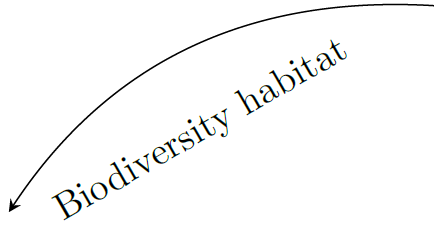
\includegraphics[width = 0.18\textwidth]{figures/wildland/arrow_biod.PNG}
    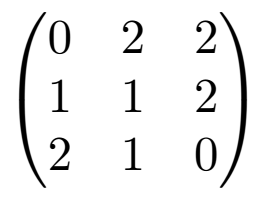
\includegraphics[width = 0.18\textwidth]{figures/wildland/land3.PNG}
    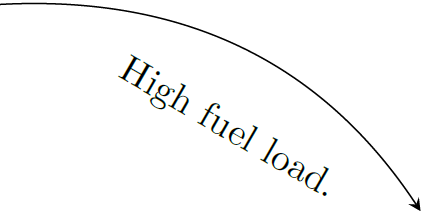
\includegraphics[width = 0.18\textwidth]{figures/wildland/arrow_fuel.PNG}
    \\
    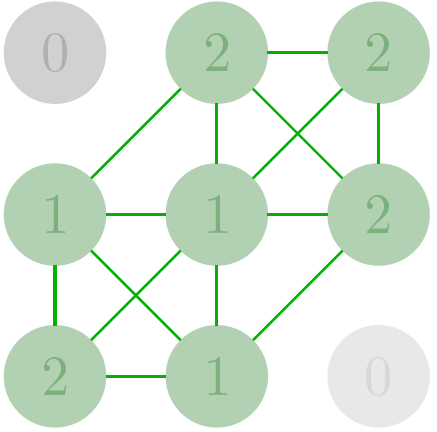
\includegraphics[width=0.2\textwidth]{figures/wildland/biodiv_3.PNG} \hspace*{4cm}
    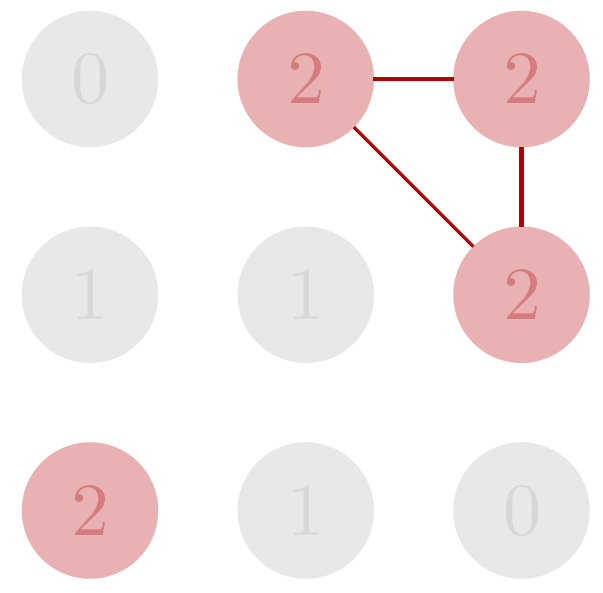
\includegraphics[width=0.2\textwidth]{figures/wildland/fire_3.PNG}\\
    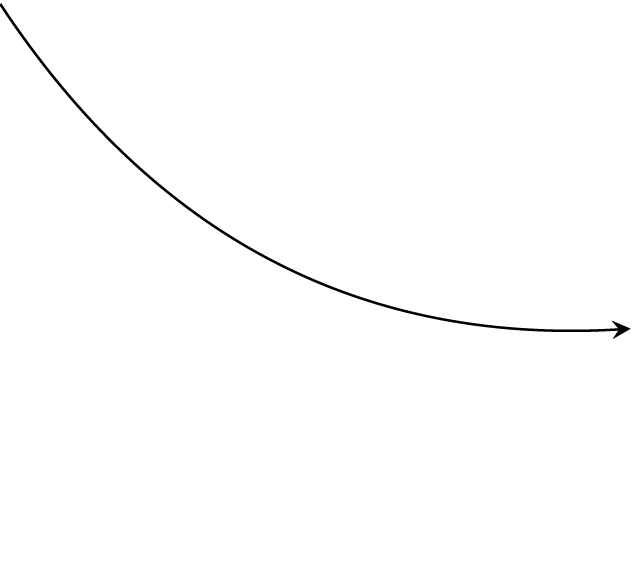
\includegraphics[width=0.18\textwidth]{figures/wildland/arrow_right.PNG}
    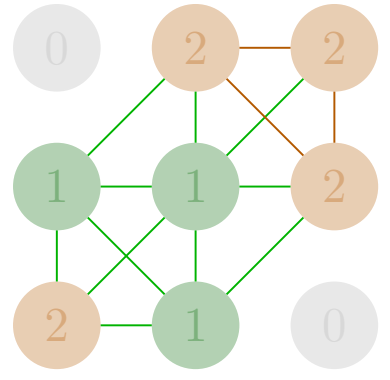
\includegraphics[width = 0.2\textwidth]{figures/wildland/graphe_feu_biod_33.PNG}
 	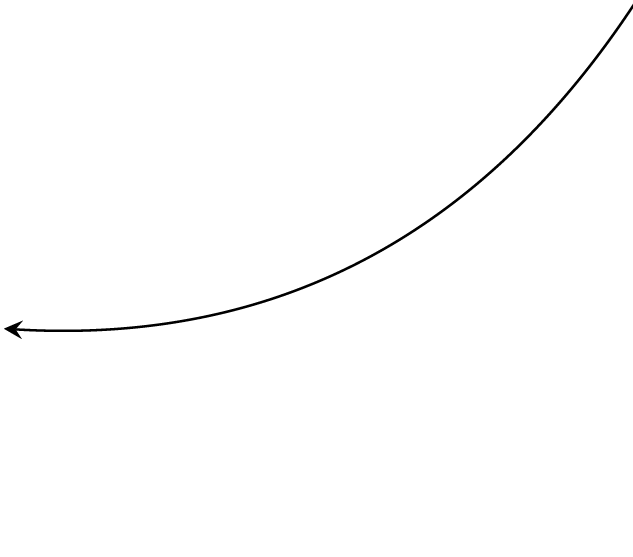
\includegraphics[width=0.18\textwidth]{figures/wildland/back_left.PNG}
    \caption{Illustration of the habitat and fuel graphs for $n=3$}
    \subcaption*{\hspace*{0.5cm}In this graph, green cells support biodiversity habitat only, while red cells display high risk. 
\\
    \hspace*{0.5cm}The high risk graph has two components (top right corner with 3 nodes, and bottom left corner with 1 node), while the biodiversity habitat graph only has one.
\\
    \hspace*{0.5cm}Cells for which the value is 0 are not considered as nodes for both graphs, and are thus not connected to the rest of the graphs. In the end, because high fuel load cells also support biodiversity habitat, the landscape can be represented as the overlap between the two graphs, where orange cells are high fuel load and also support biodiversity habitat.}

    \label{fig:graph_overlap}
\end{figure}

\newpage
\begin{figure}[H]
    \centering
    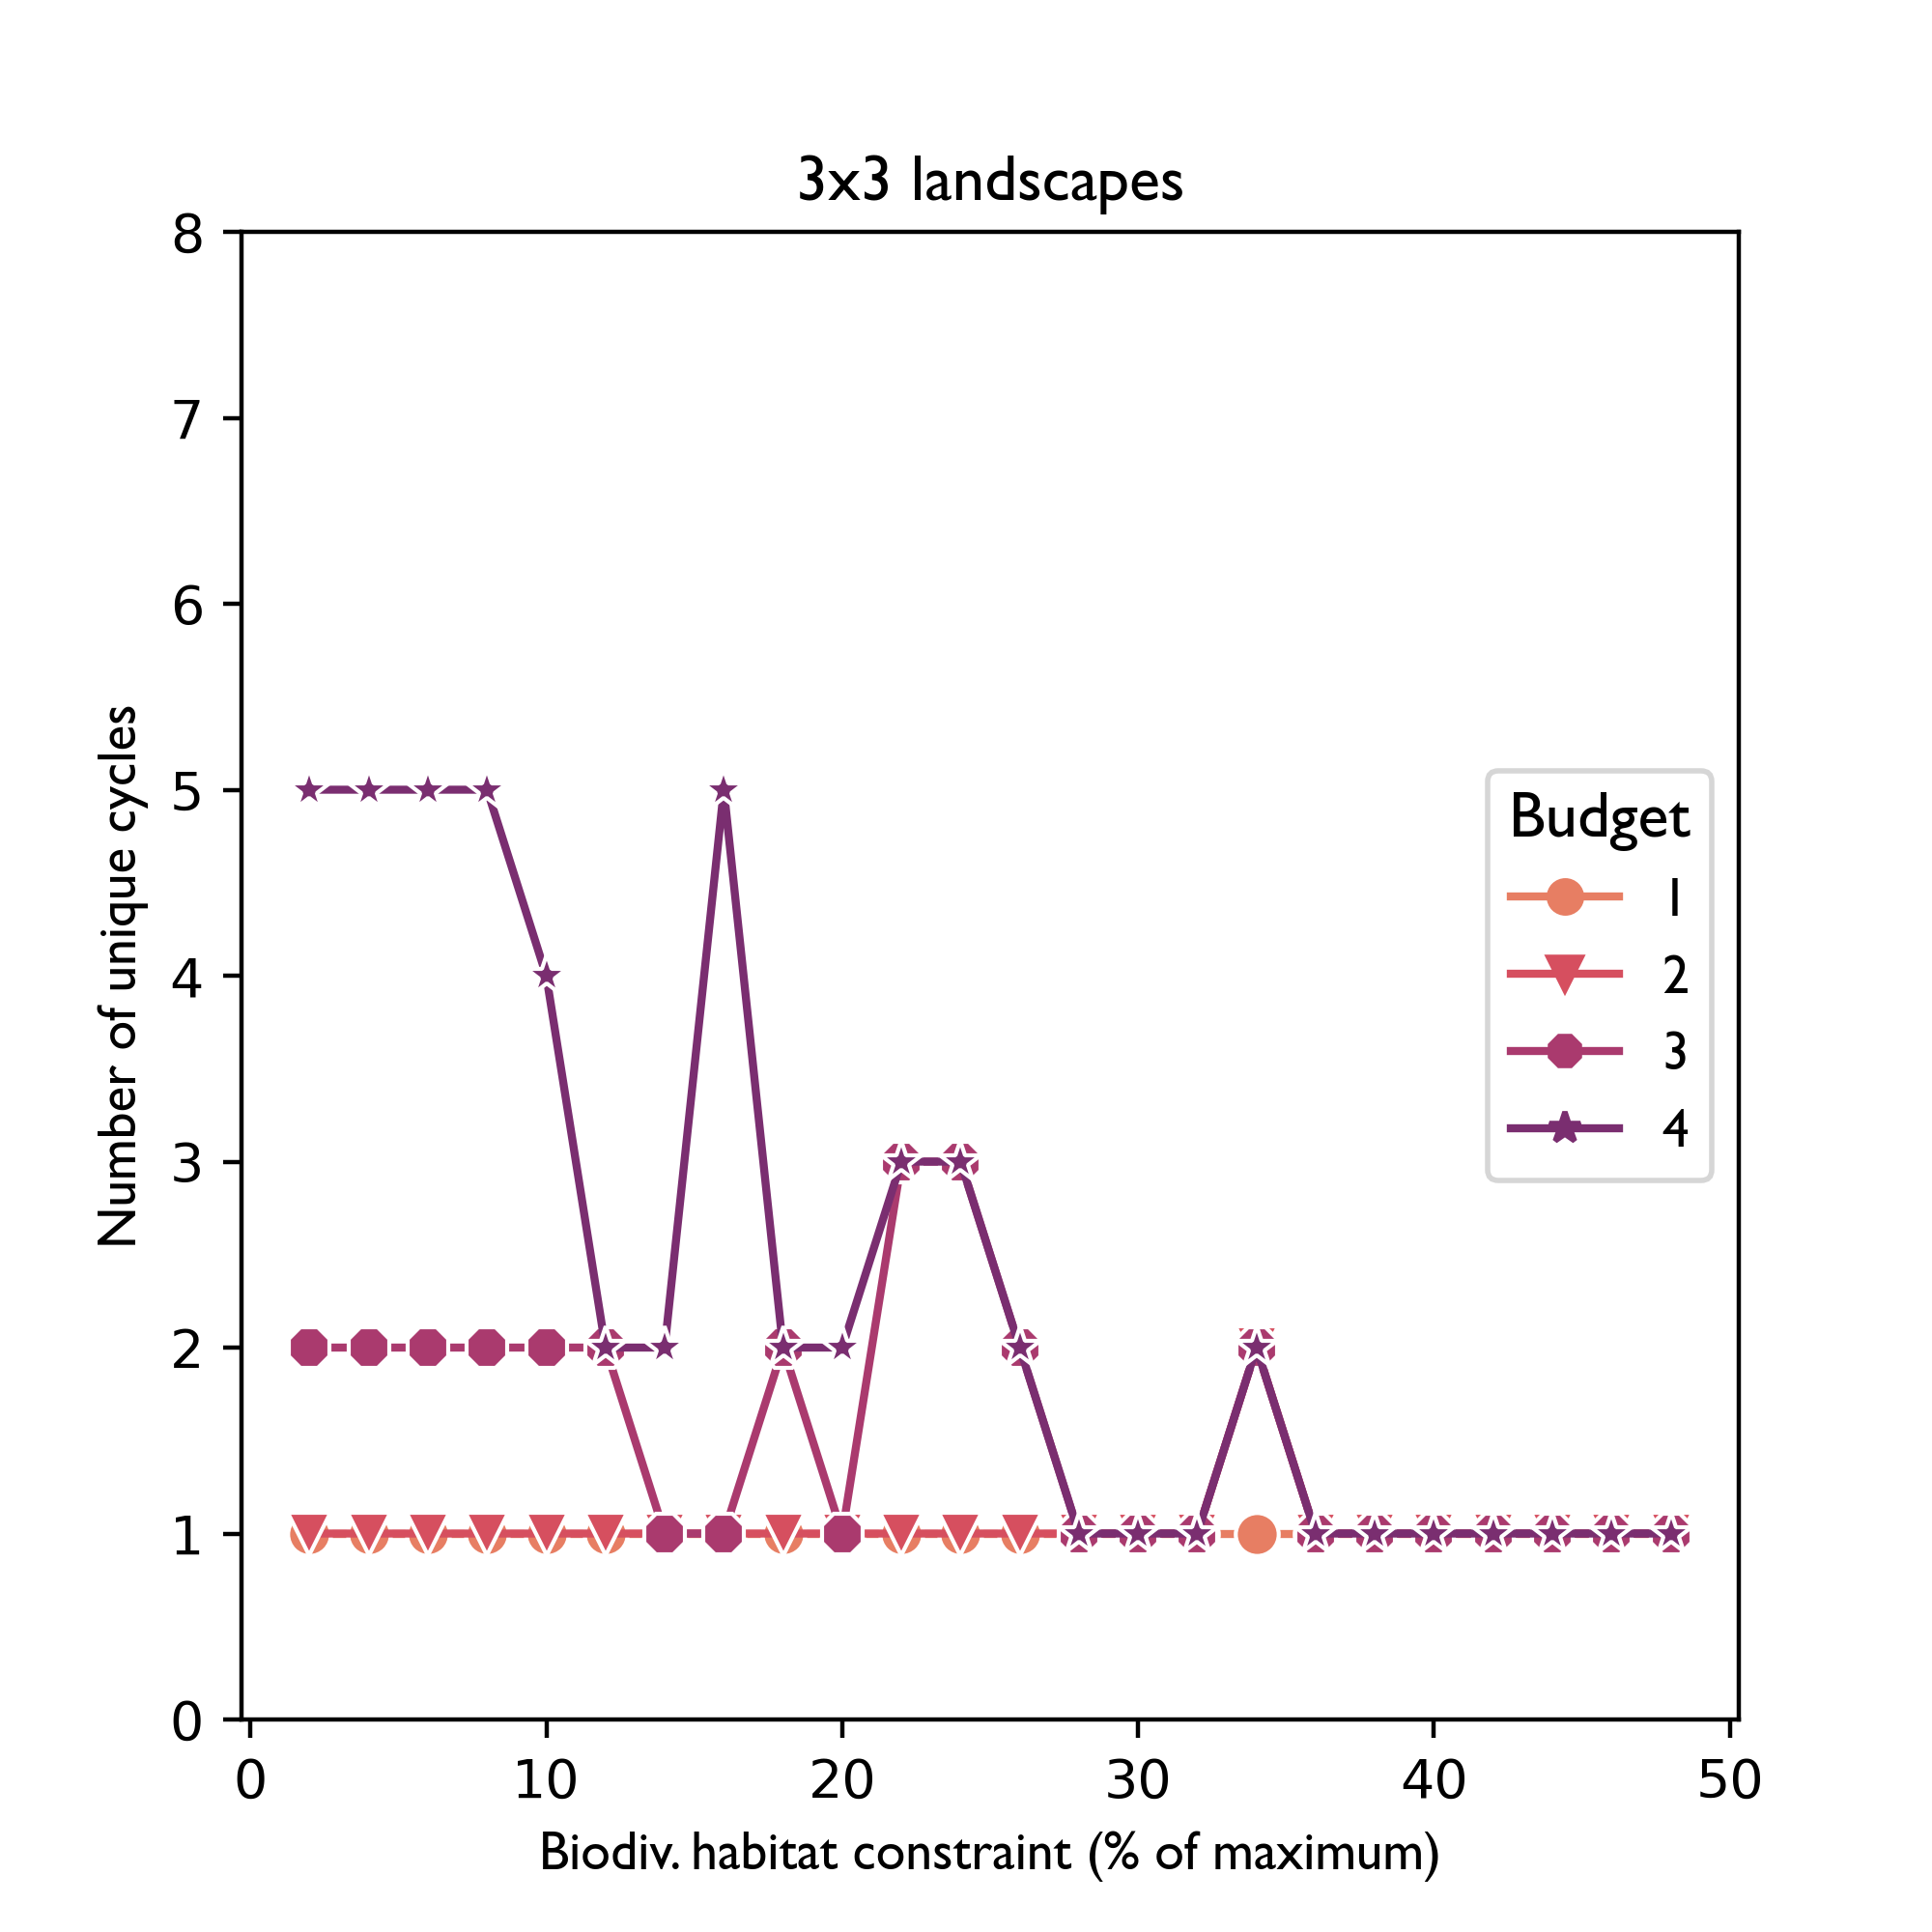
\includegraphics[width = 0.45\textwidth]{figures/wildland/number_cycles3.png}
    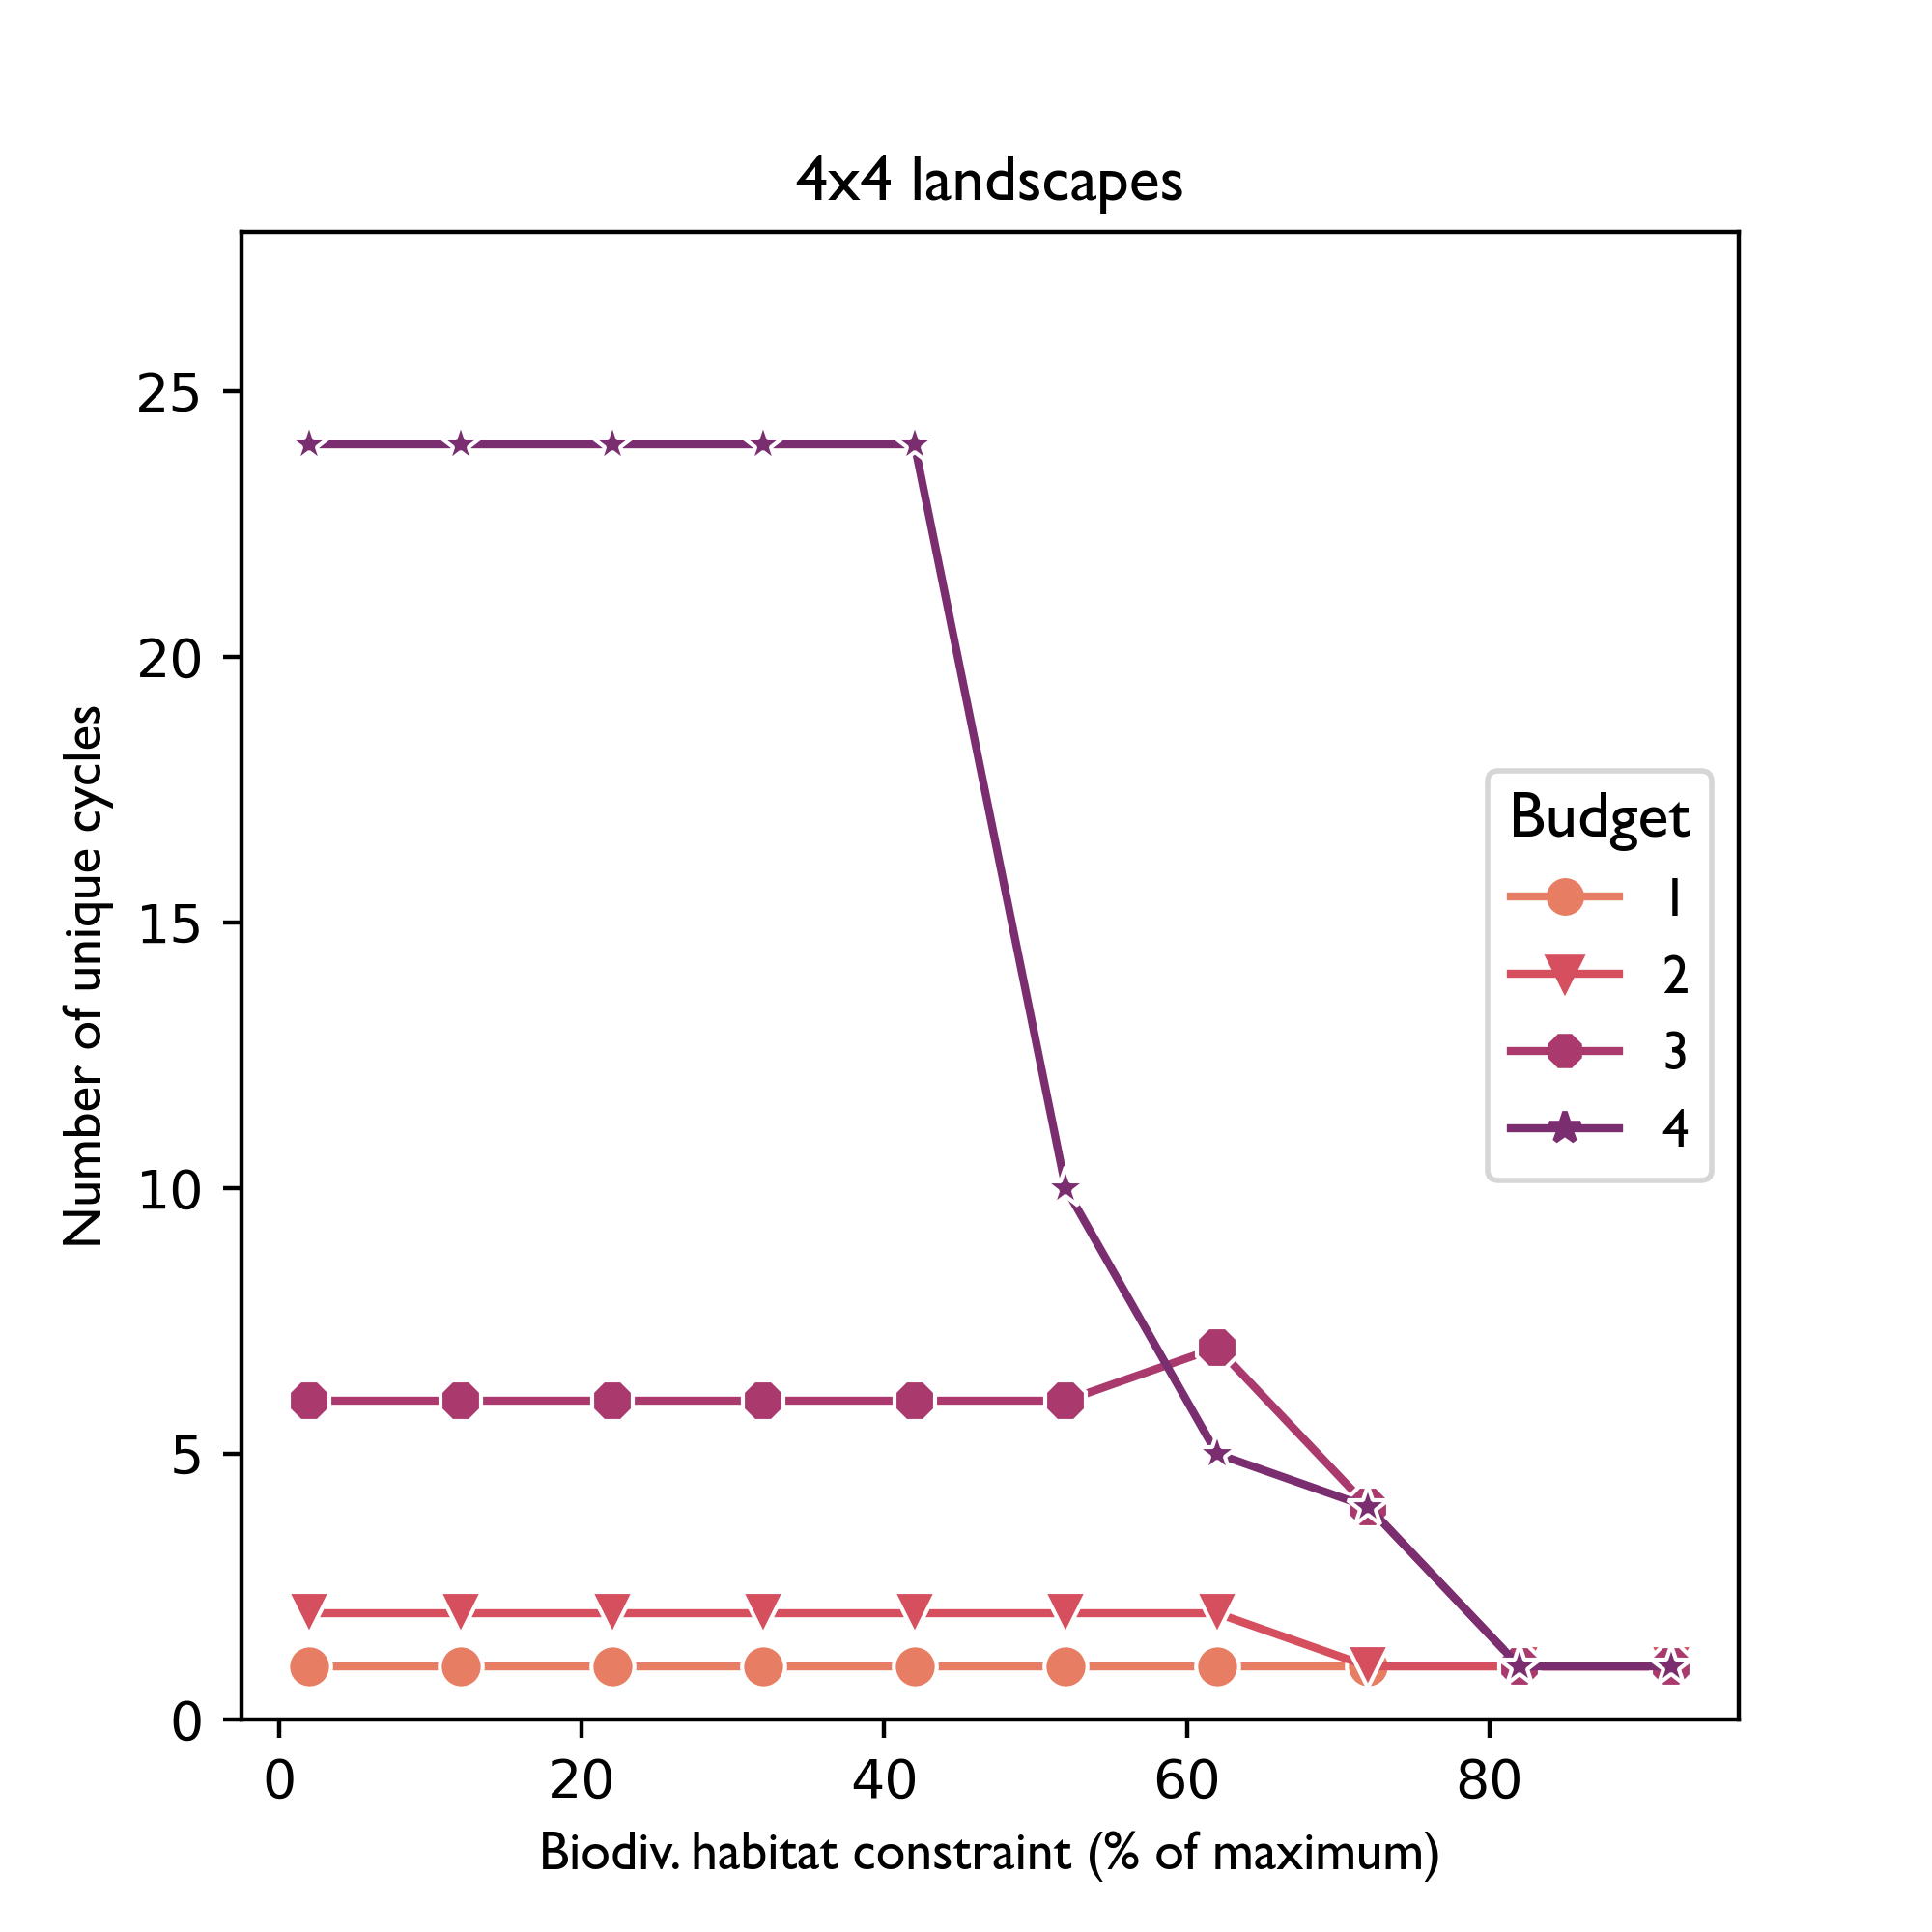
\includegraphics[width = 0.45\textwidth]{figures/wildland/number_cycles4.png}
    \caption{Number of cycles as a function of biodiversity habitat and budget}
    \label{fig:distrib_cycles}
\end{figure}
\newpage
\begin{figure}[h]
    \centering
    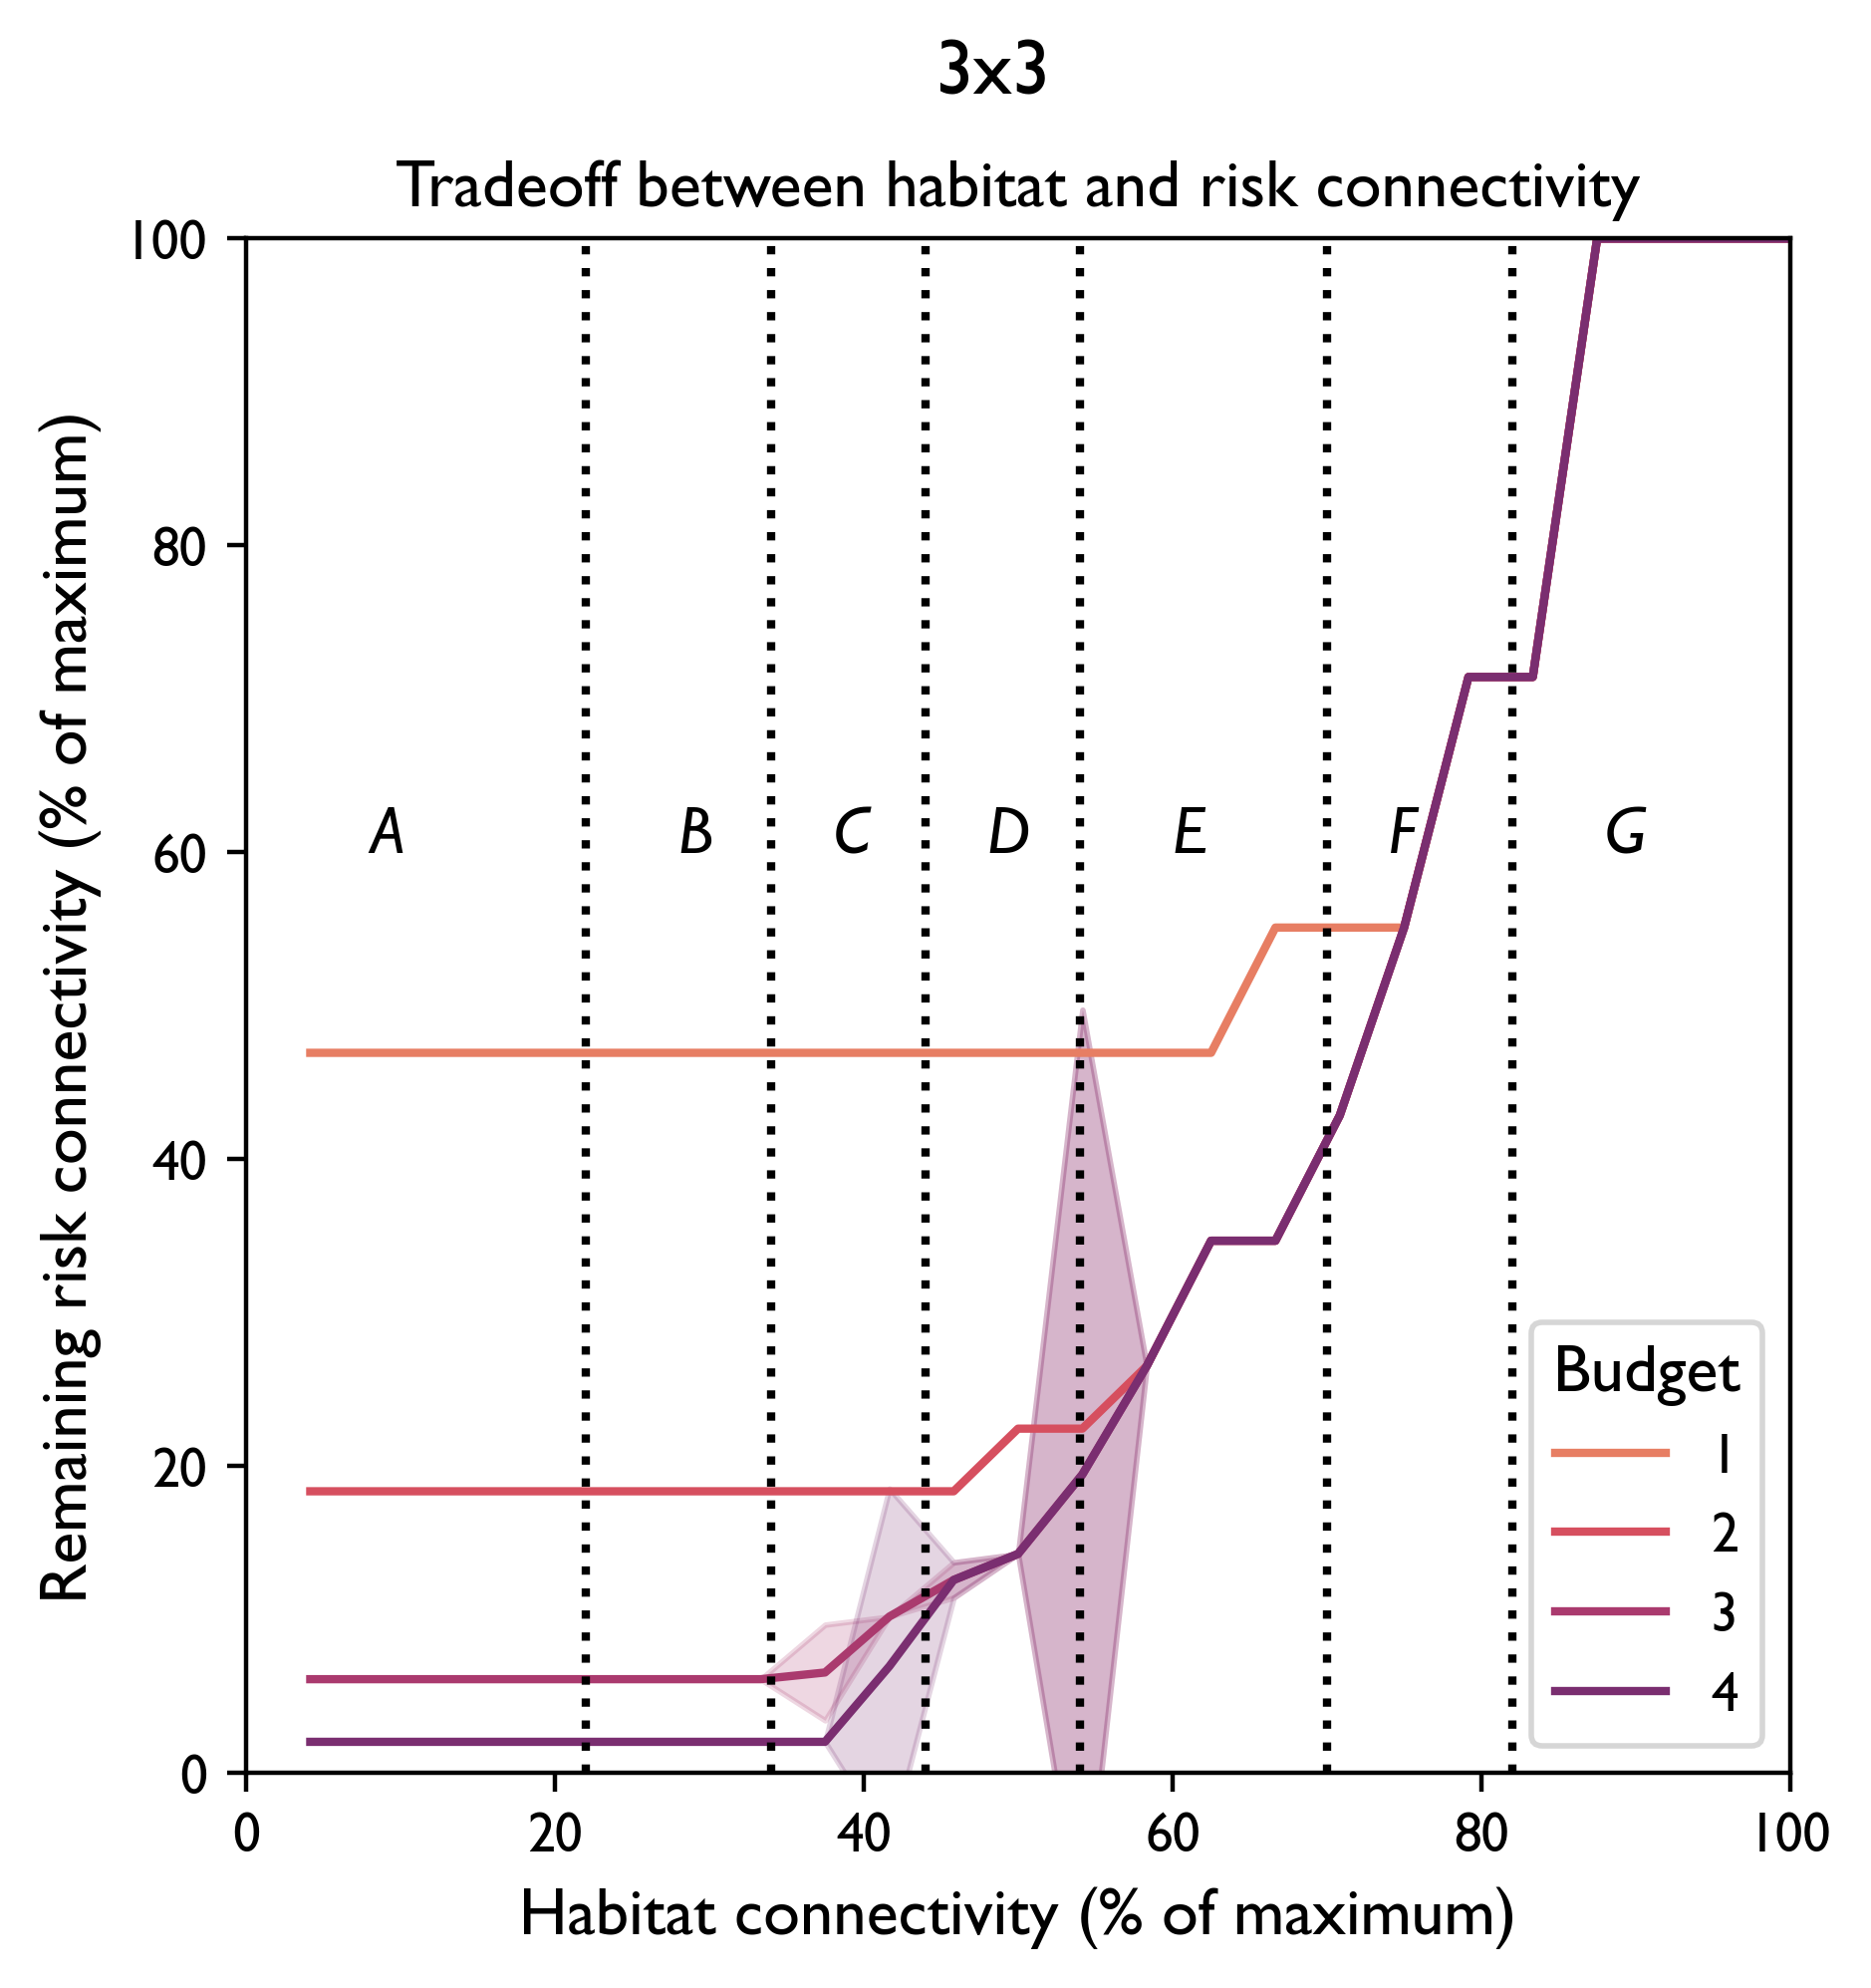
\includegraphics[width=0.5\textwidth]{figures/wildland/tradeoff3.png}\hfill
    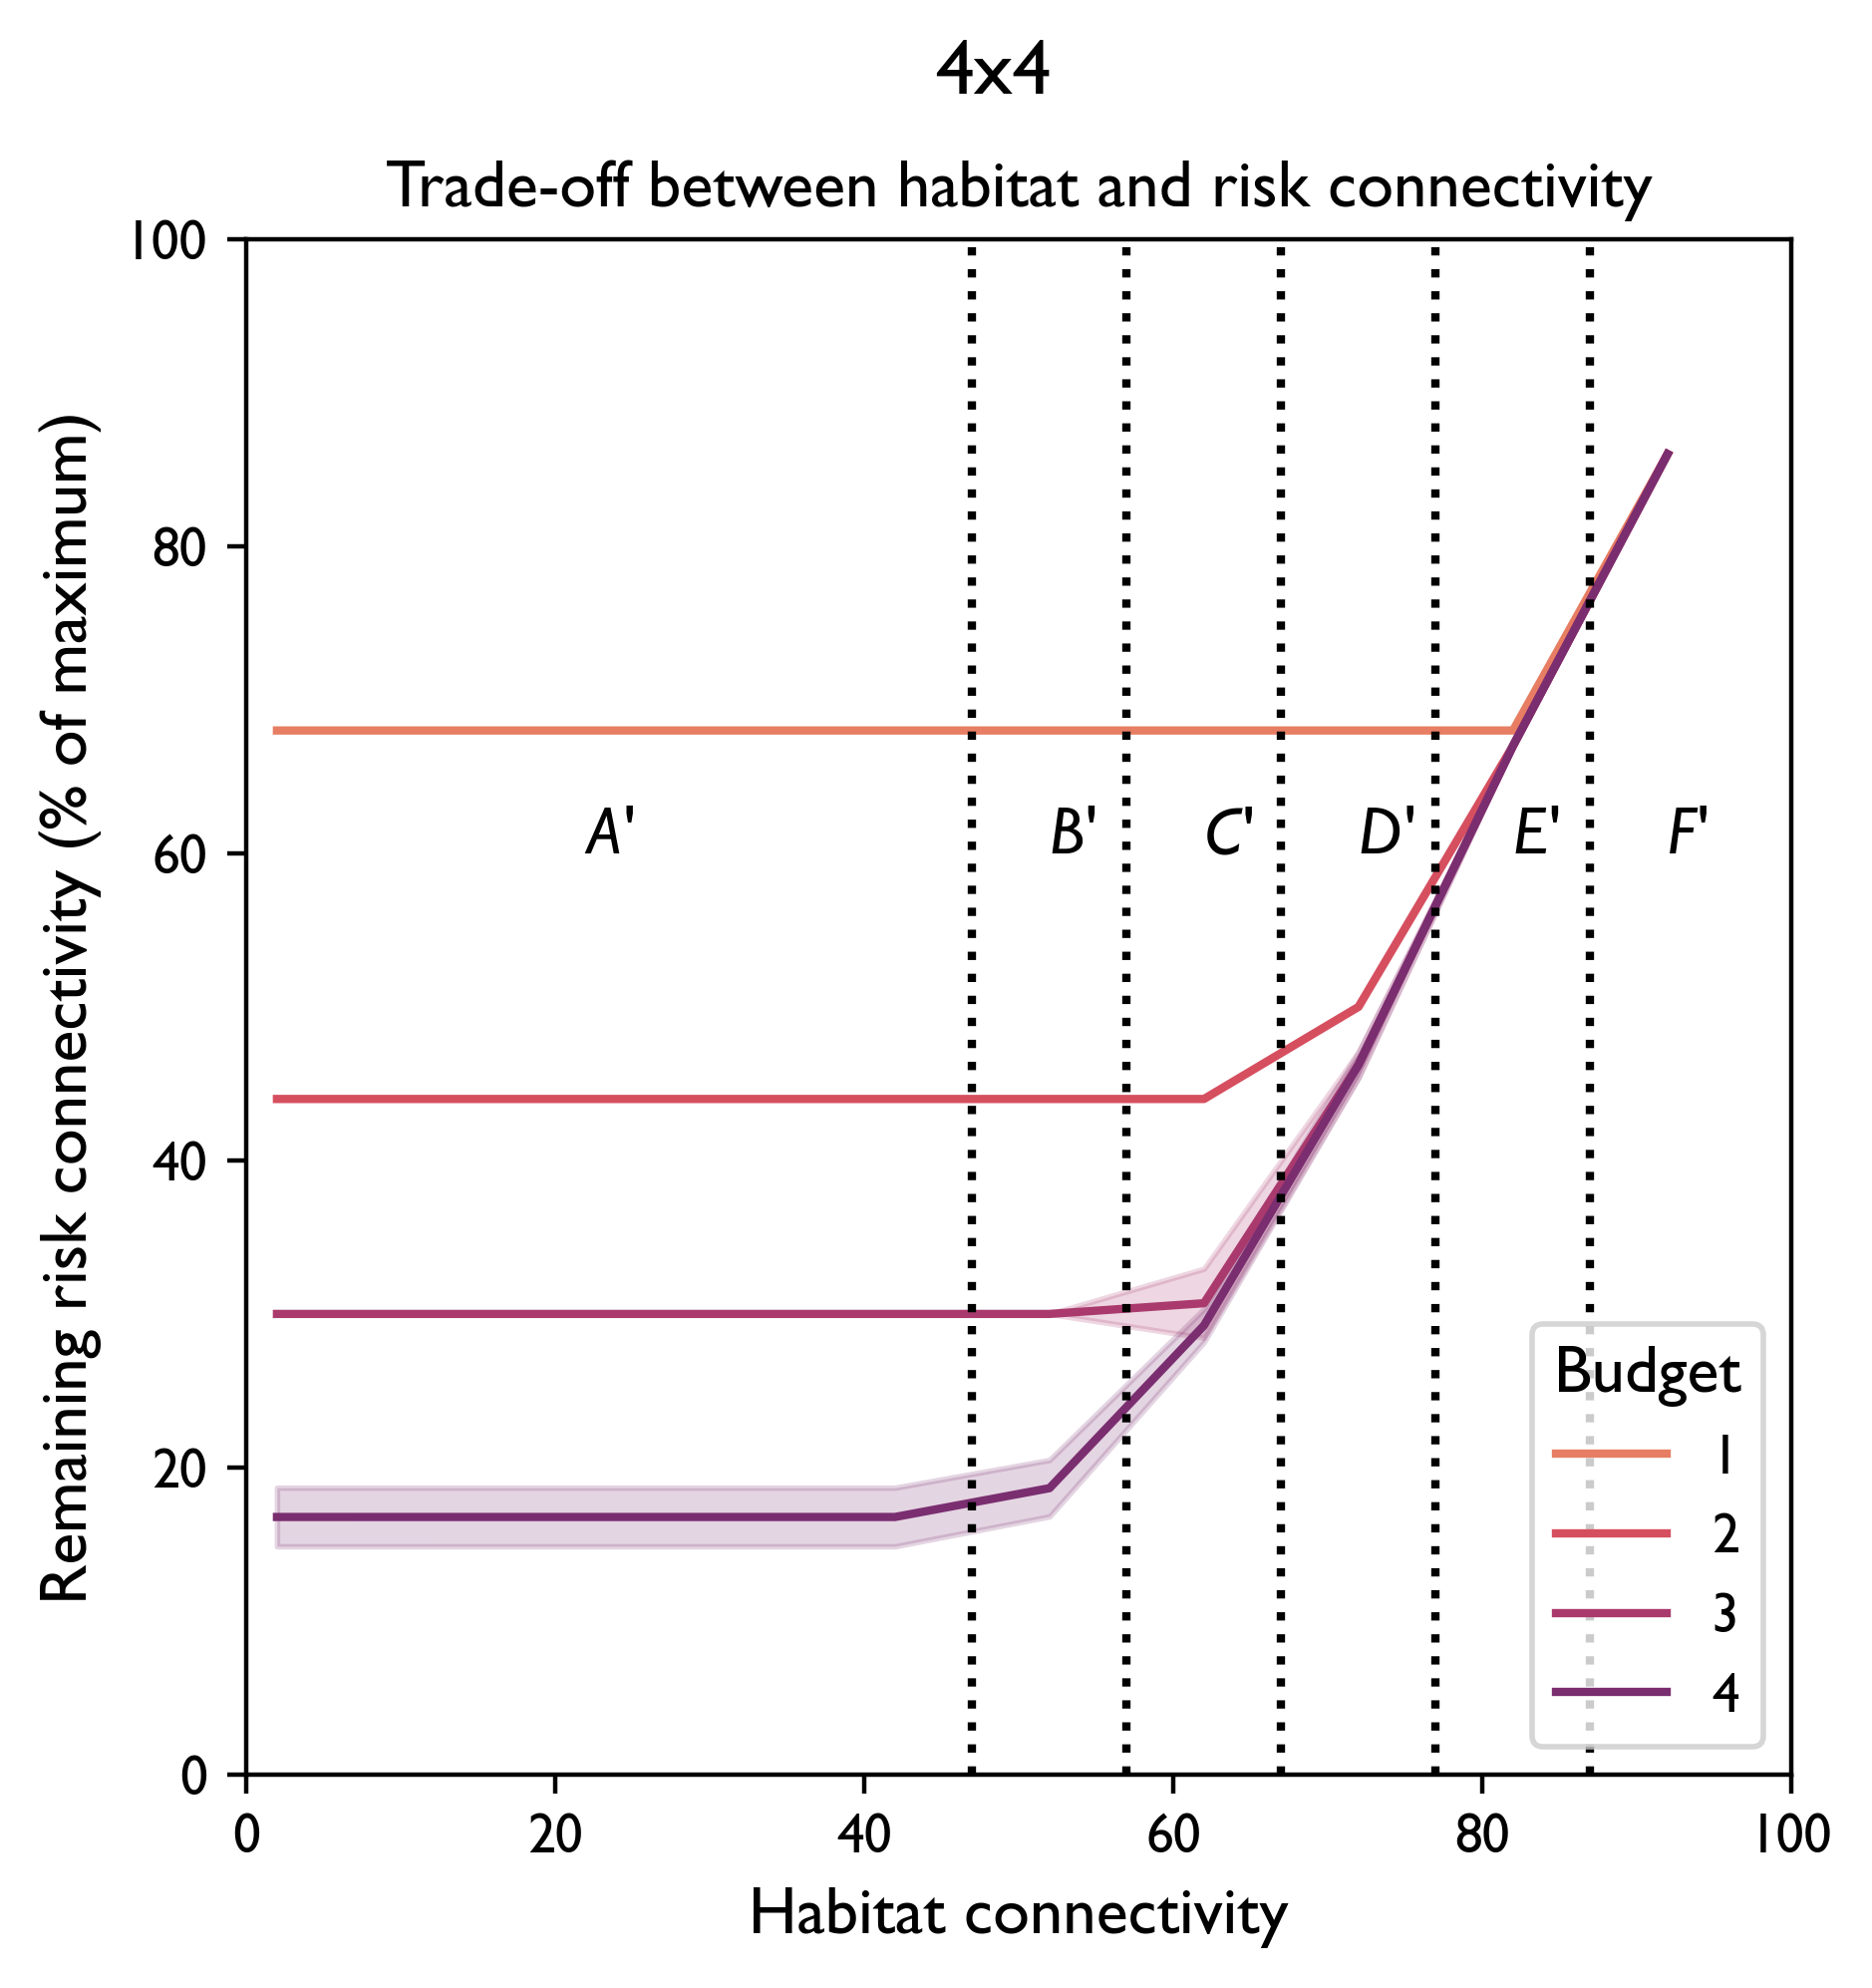
\includegraphics[width=0.5\textwidth]{figures/wildland/tradeoff4.png}
    \\[\smallskipamount]
    \caption{Production possibility frontier between constraint (as a \% of maximum biodiversity sustainable in landscape) and wildfire risk for various budgets, and landscape size}
    \label{fig:frontier}
\end{figure}
\newpage

% Landscapes 
\begin{figure}[H]
    \centering
    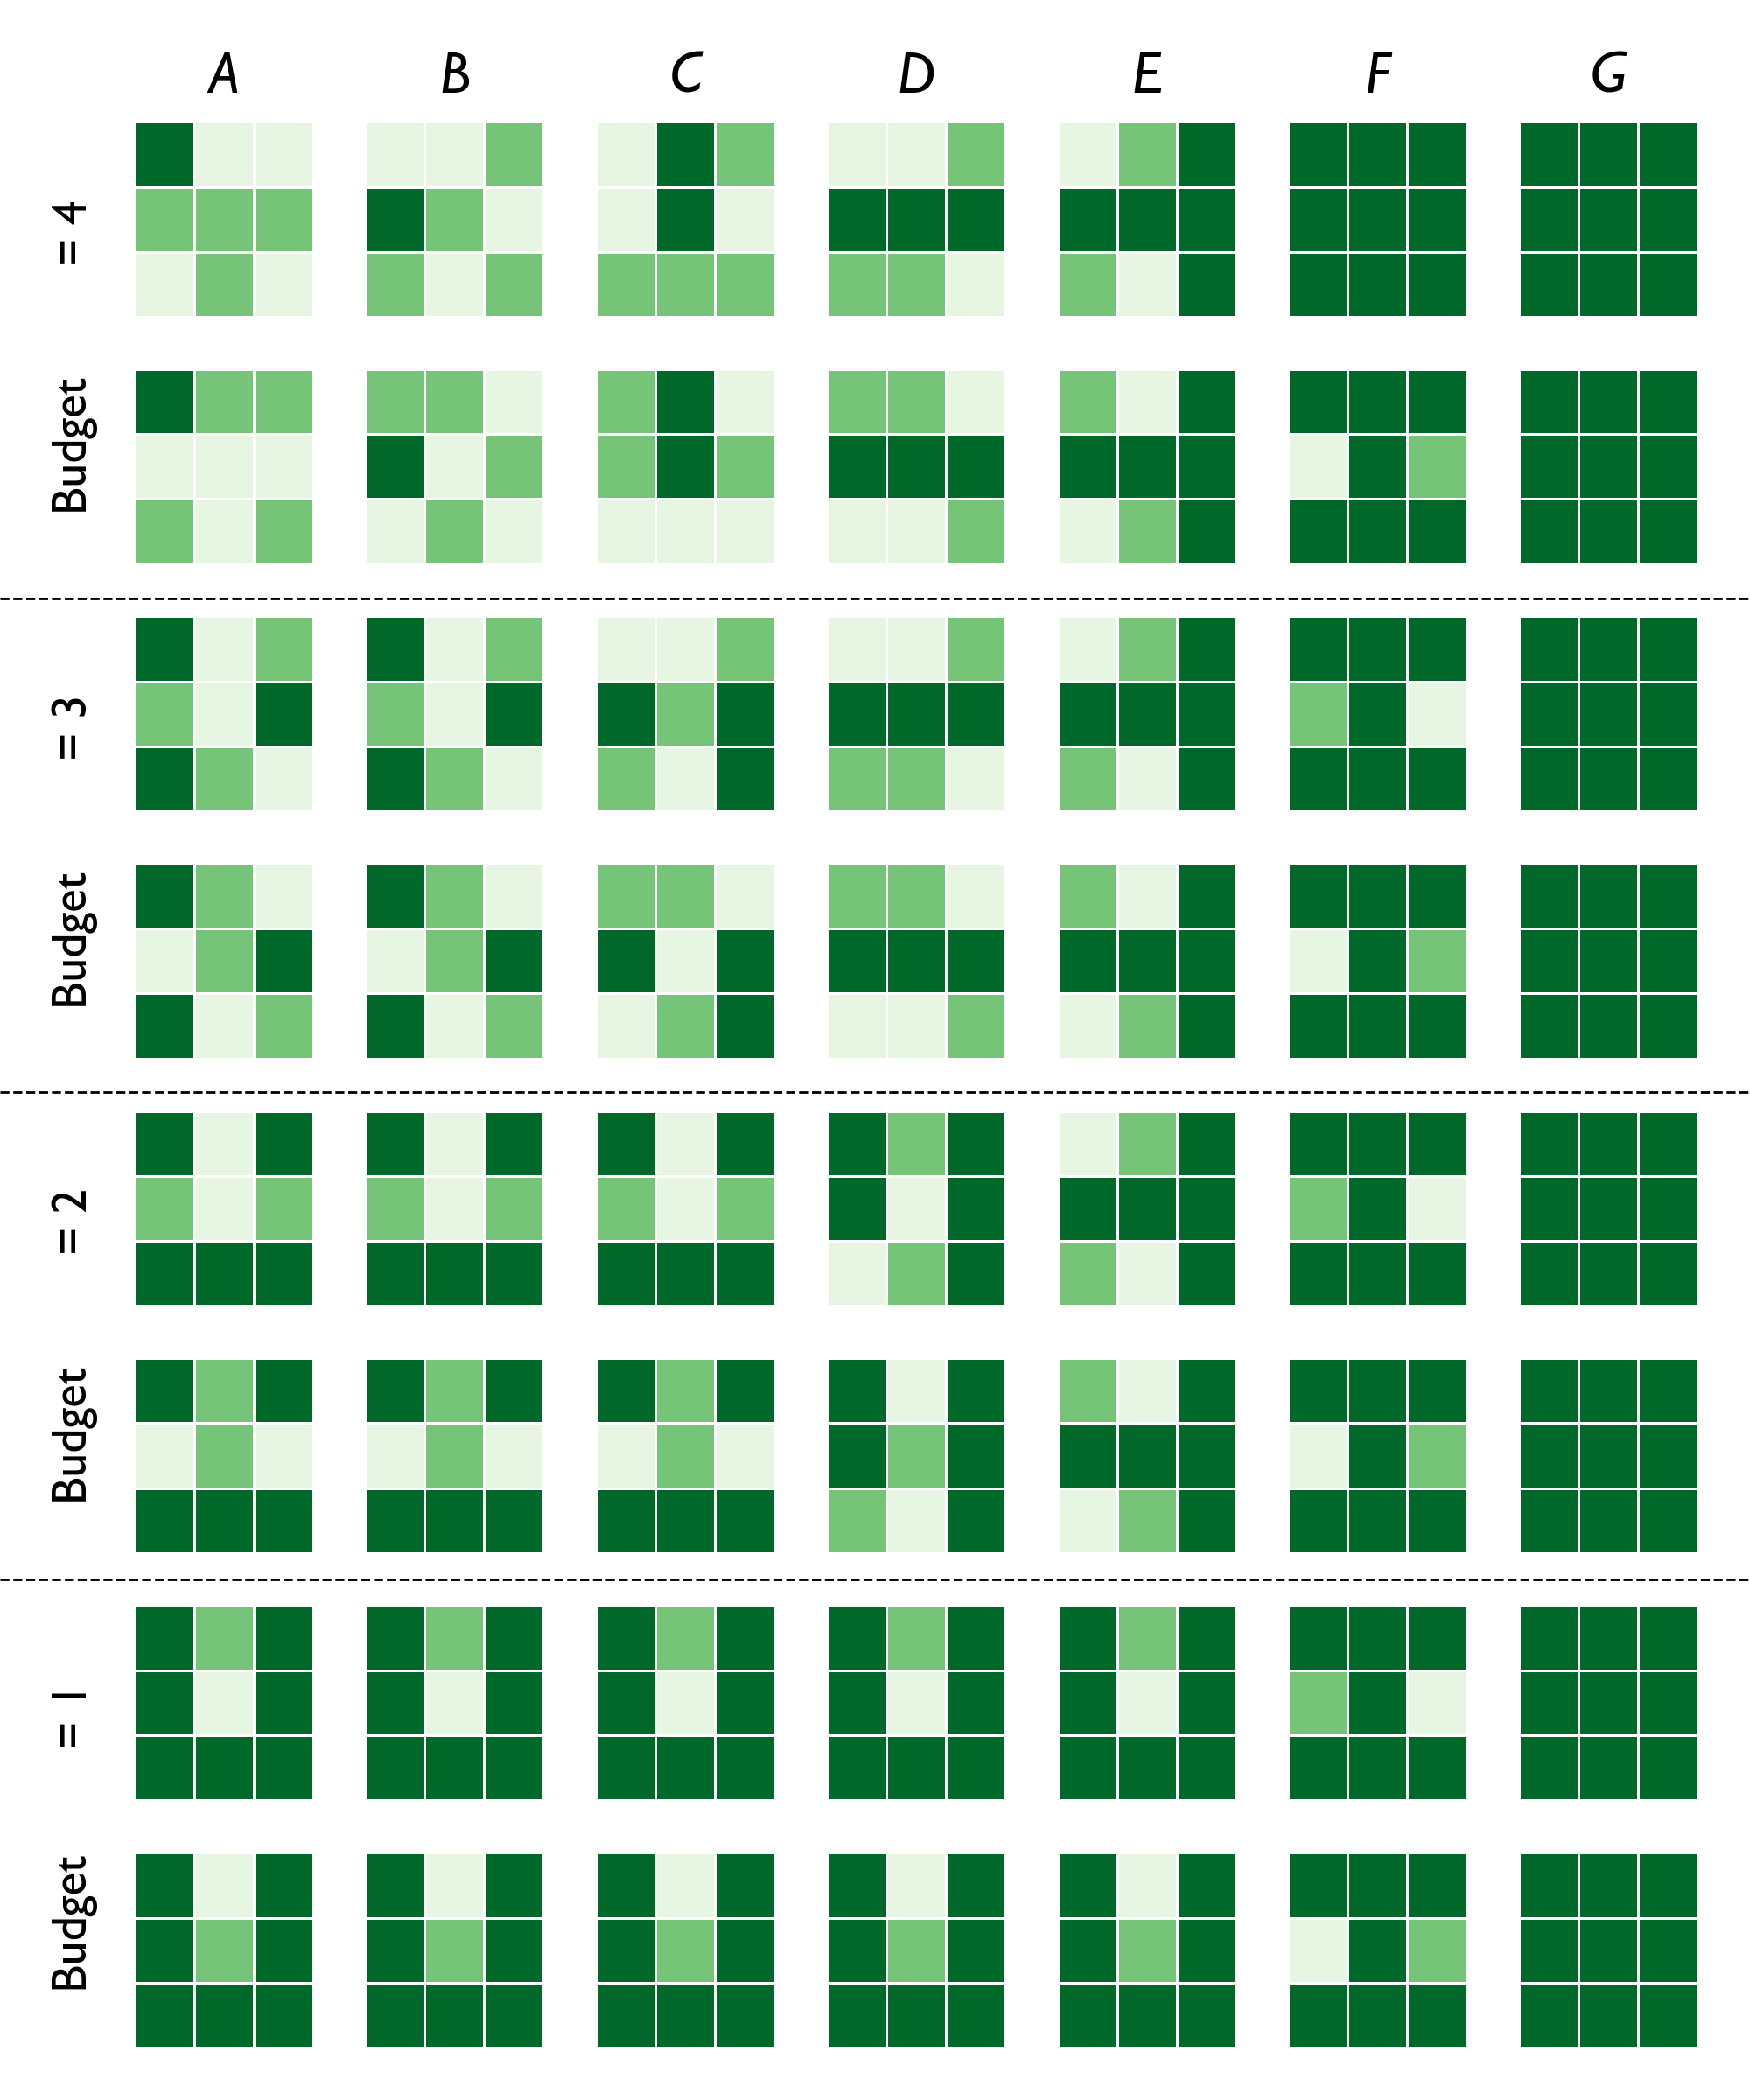
\includegraphics[width=0.40\textwidth, height=9cm]{figures/wildland/landscapes3.png}
    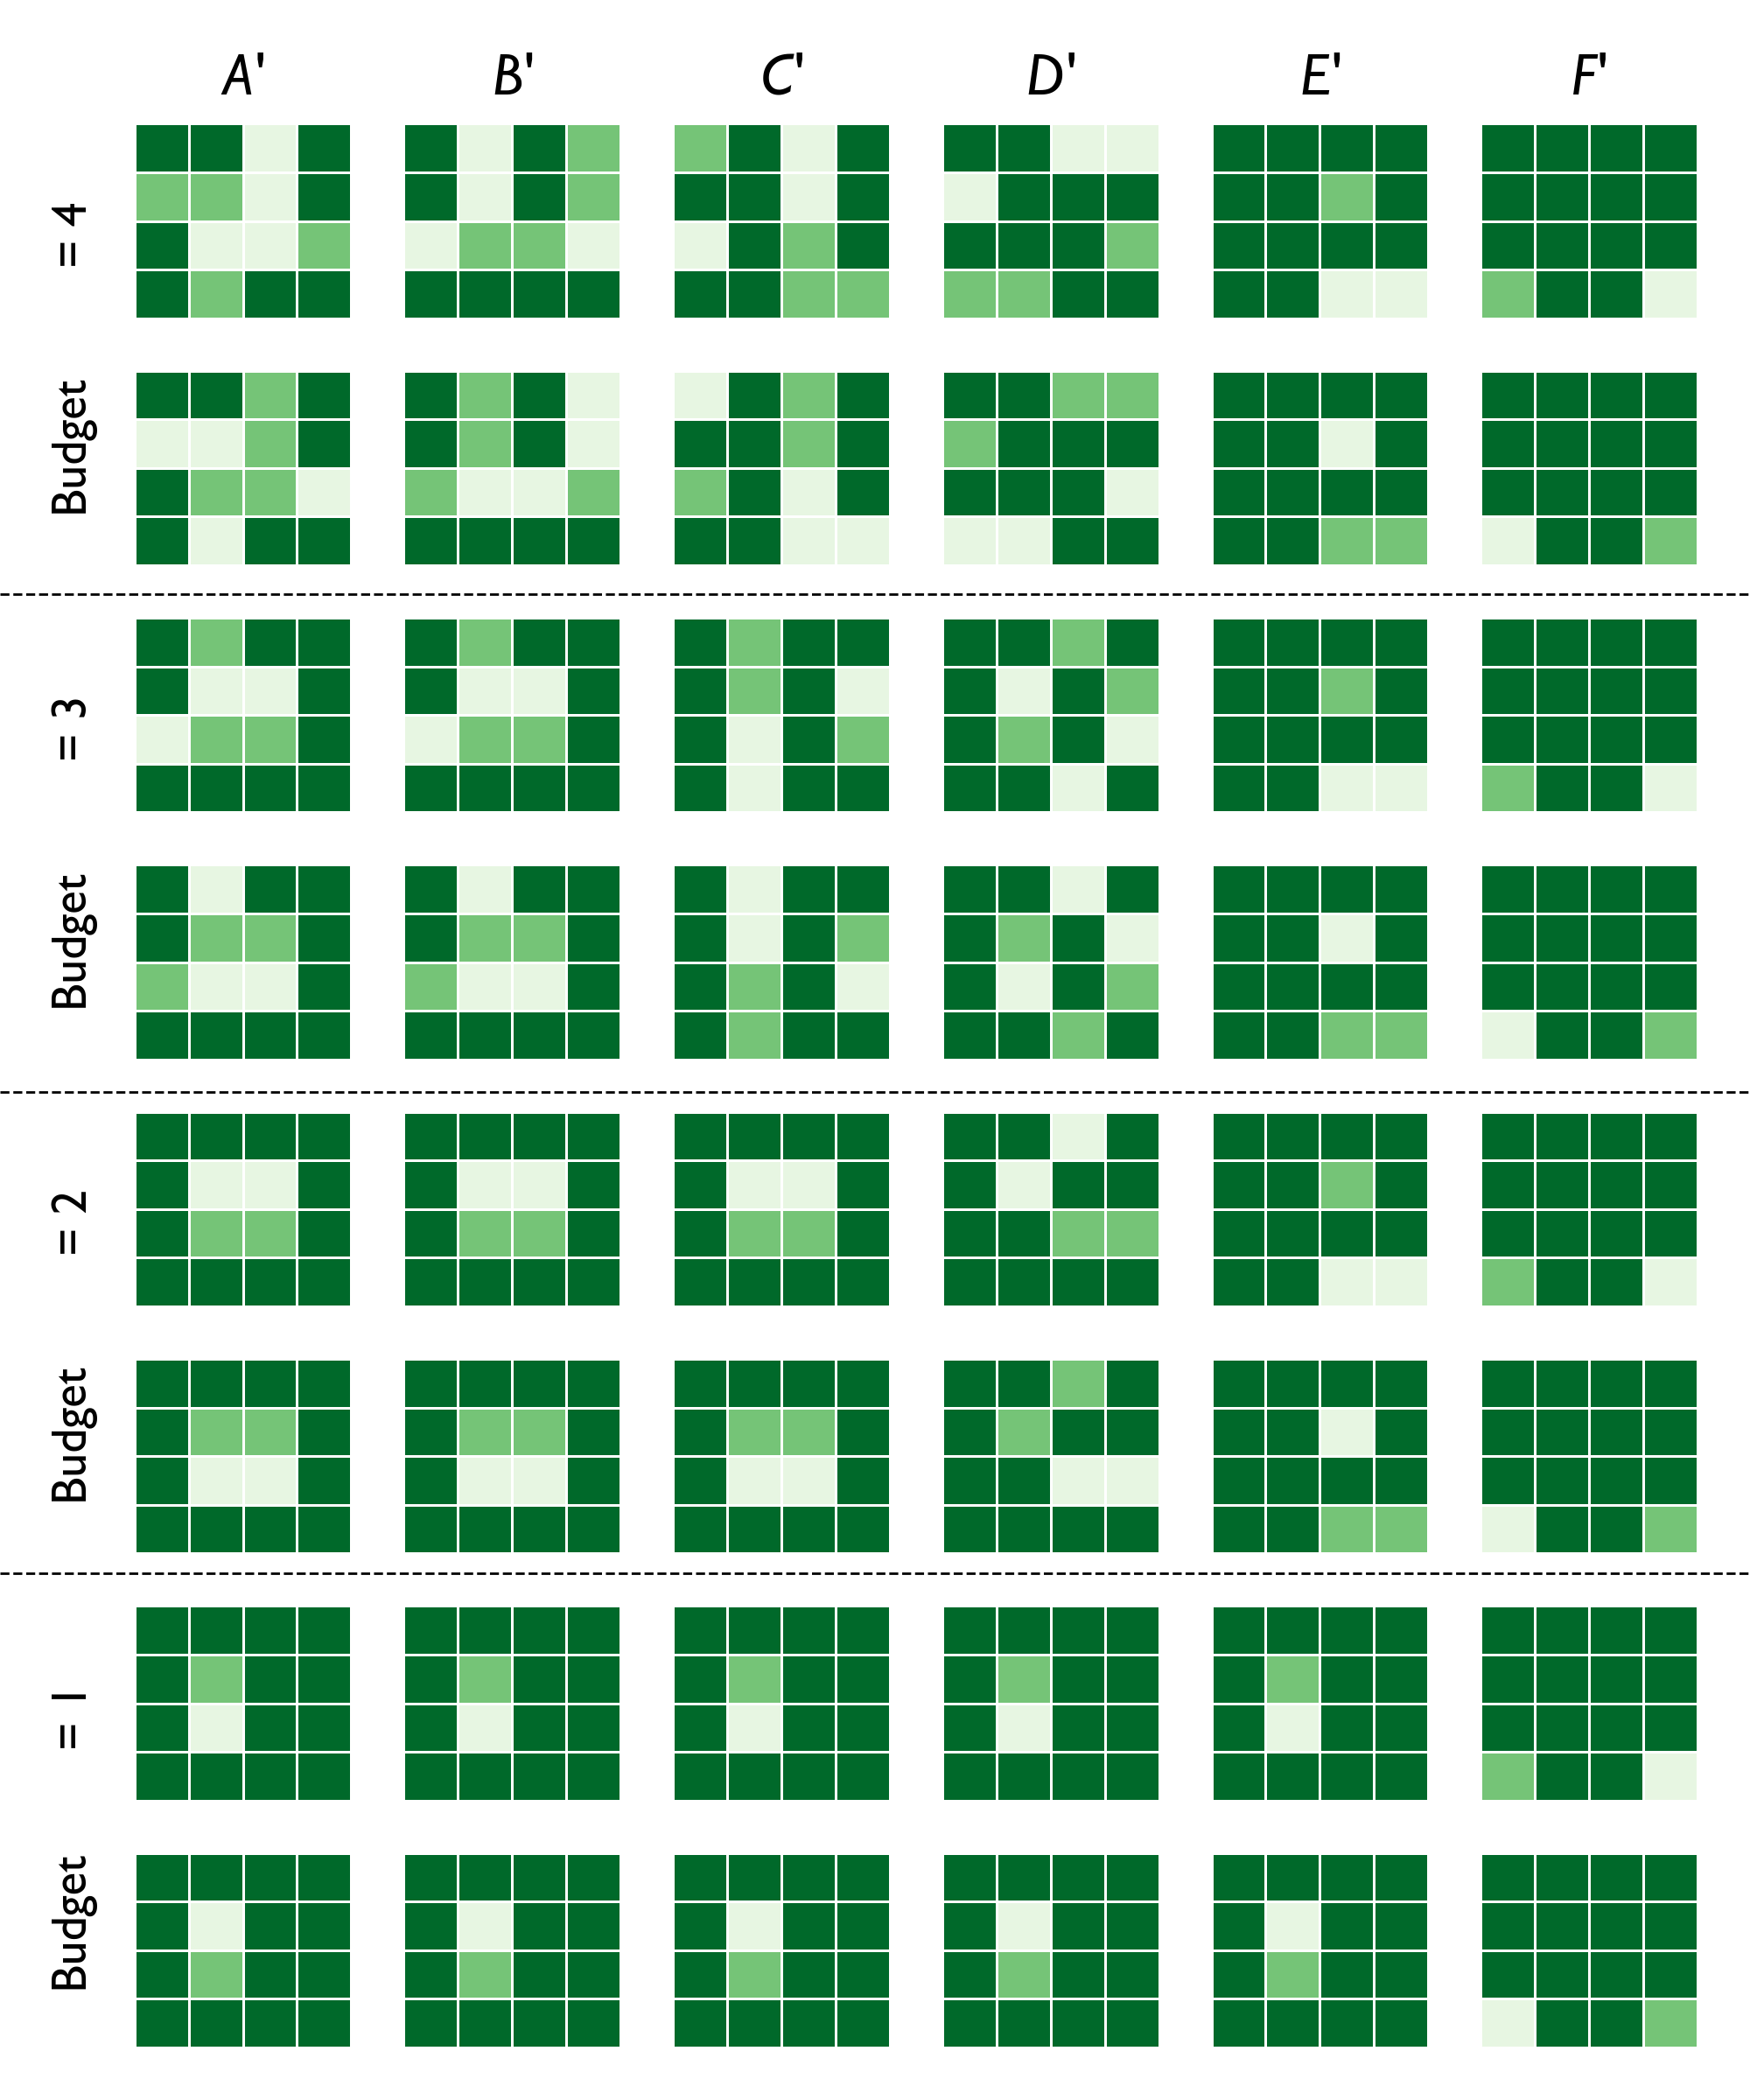
\includegraphics[width=0.45\textwidth, height=10cm]{figures/wildland/landscapes4.png}
    \caption{Most represented cycles for each biodiversity constraint level, for various budget and landscapes $3 \times 3$, and $4\times 4$ (95\% CI shaded)}
    \label{fig:cycles_3_4}
\end{figure}
\newpage

\begin{figure}[H]
     \centering
     \begin{subfigure}[b]{0.4\textwidth}
         \centering
         \includegraphics[width=.98\textwidth]{figures/wildland/risky_surface3.png}
         \caption{}
         \label{fig:indicator_surface3}
     \end{subfigure}
     \begin{subfigure}[b]{0.4\textwidth}
         \centering
         \includegraphics[width=\textwidth]{figures/wildland/risky_surface4.png}
         \caption{}
         \label{fig:indicator_surface4}
     \end{subfigure}
     \hfill
     \begin{subfigure}[b]{0.4\textwidth}
         \centering
         \includegraphics[width=\textwidth]{figures/wildland/risky_components3.png}
         \caption{}
         \label{fig:indicator_component3}
     \end{subfigure}
     \begin{subfigure}[b]{0.4\textwidth}
         \centering
         \includegraphics[width=.98\textwidth]{figures/wildland/risky_component4.png}
         \caption{}
         \label{fig:indicator_component4}
     \end{subfigure}
     \hfill
          \begin{subfigure}[b]{0.4\textwidth}
         \centering
         \includegraphics[width=.98\textwidth]{figures/wildland/max_component_area3.png}
         \caption{}
         \label{fig:indicator_component3}
     \end{subfigure}
     \begin{subfigure}[b]{0.4\textwidth}
         \centering
         \includegraphics[width=\textwidth]{figures/wildland/max_component_area4.png}
         \caption{}
         \label{fig:indicator_component4}
     \end{subfigure}
        \caption{Assessment: surface, components of high-risk graph (95\% CI shaded)}
        \label{fig:indicators_1}
\end{figure}
\newpage

%\begin{figure}[H]
%    \centering
%    \includegraphics[width=0.45\textwidth]{squelette_draft/graphs_manuscript/risky_surface3.png} 
%    \includegraphics[width=0.45\textwidth]{squelette_draft/graphs_manuscript/risky_surface4.png}\\
%    \includegraphics[width=0.45\textwidth]{squelette_draft/graphs_manuscript/risky_components3.png}
%    \includegraphics[width=0.45\textwidth]{squelette_draft/graphs_manuscript/risky_component4.png}\\
%    \includegraphics[width=0.45\textwidth]{squelette_draft/graphs_manuscript/max_component_area3.png} 
%    \includegraphics[width=0.45\textwidth]{squelette_draft/graphs_manuscript/max_component_area4.png} 
%    \caption{Assessment indicators: surface and components of high-risk graph}
%    \label{fig:indicators_1}
%\end{figure}

\begin{figure}[H]
     \centering
     \begin{subfigure}[b]{0.4\textwidth}
         \centering
         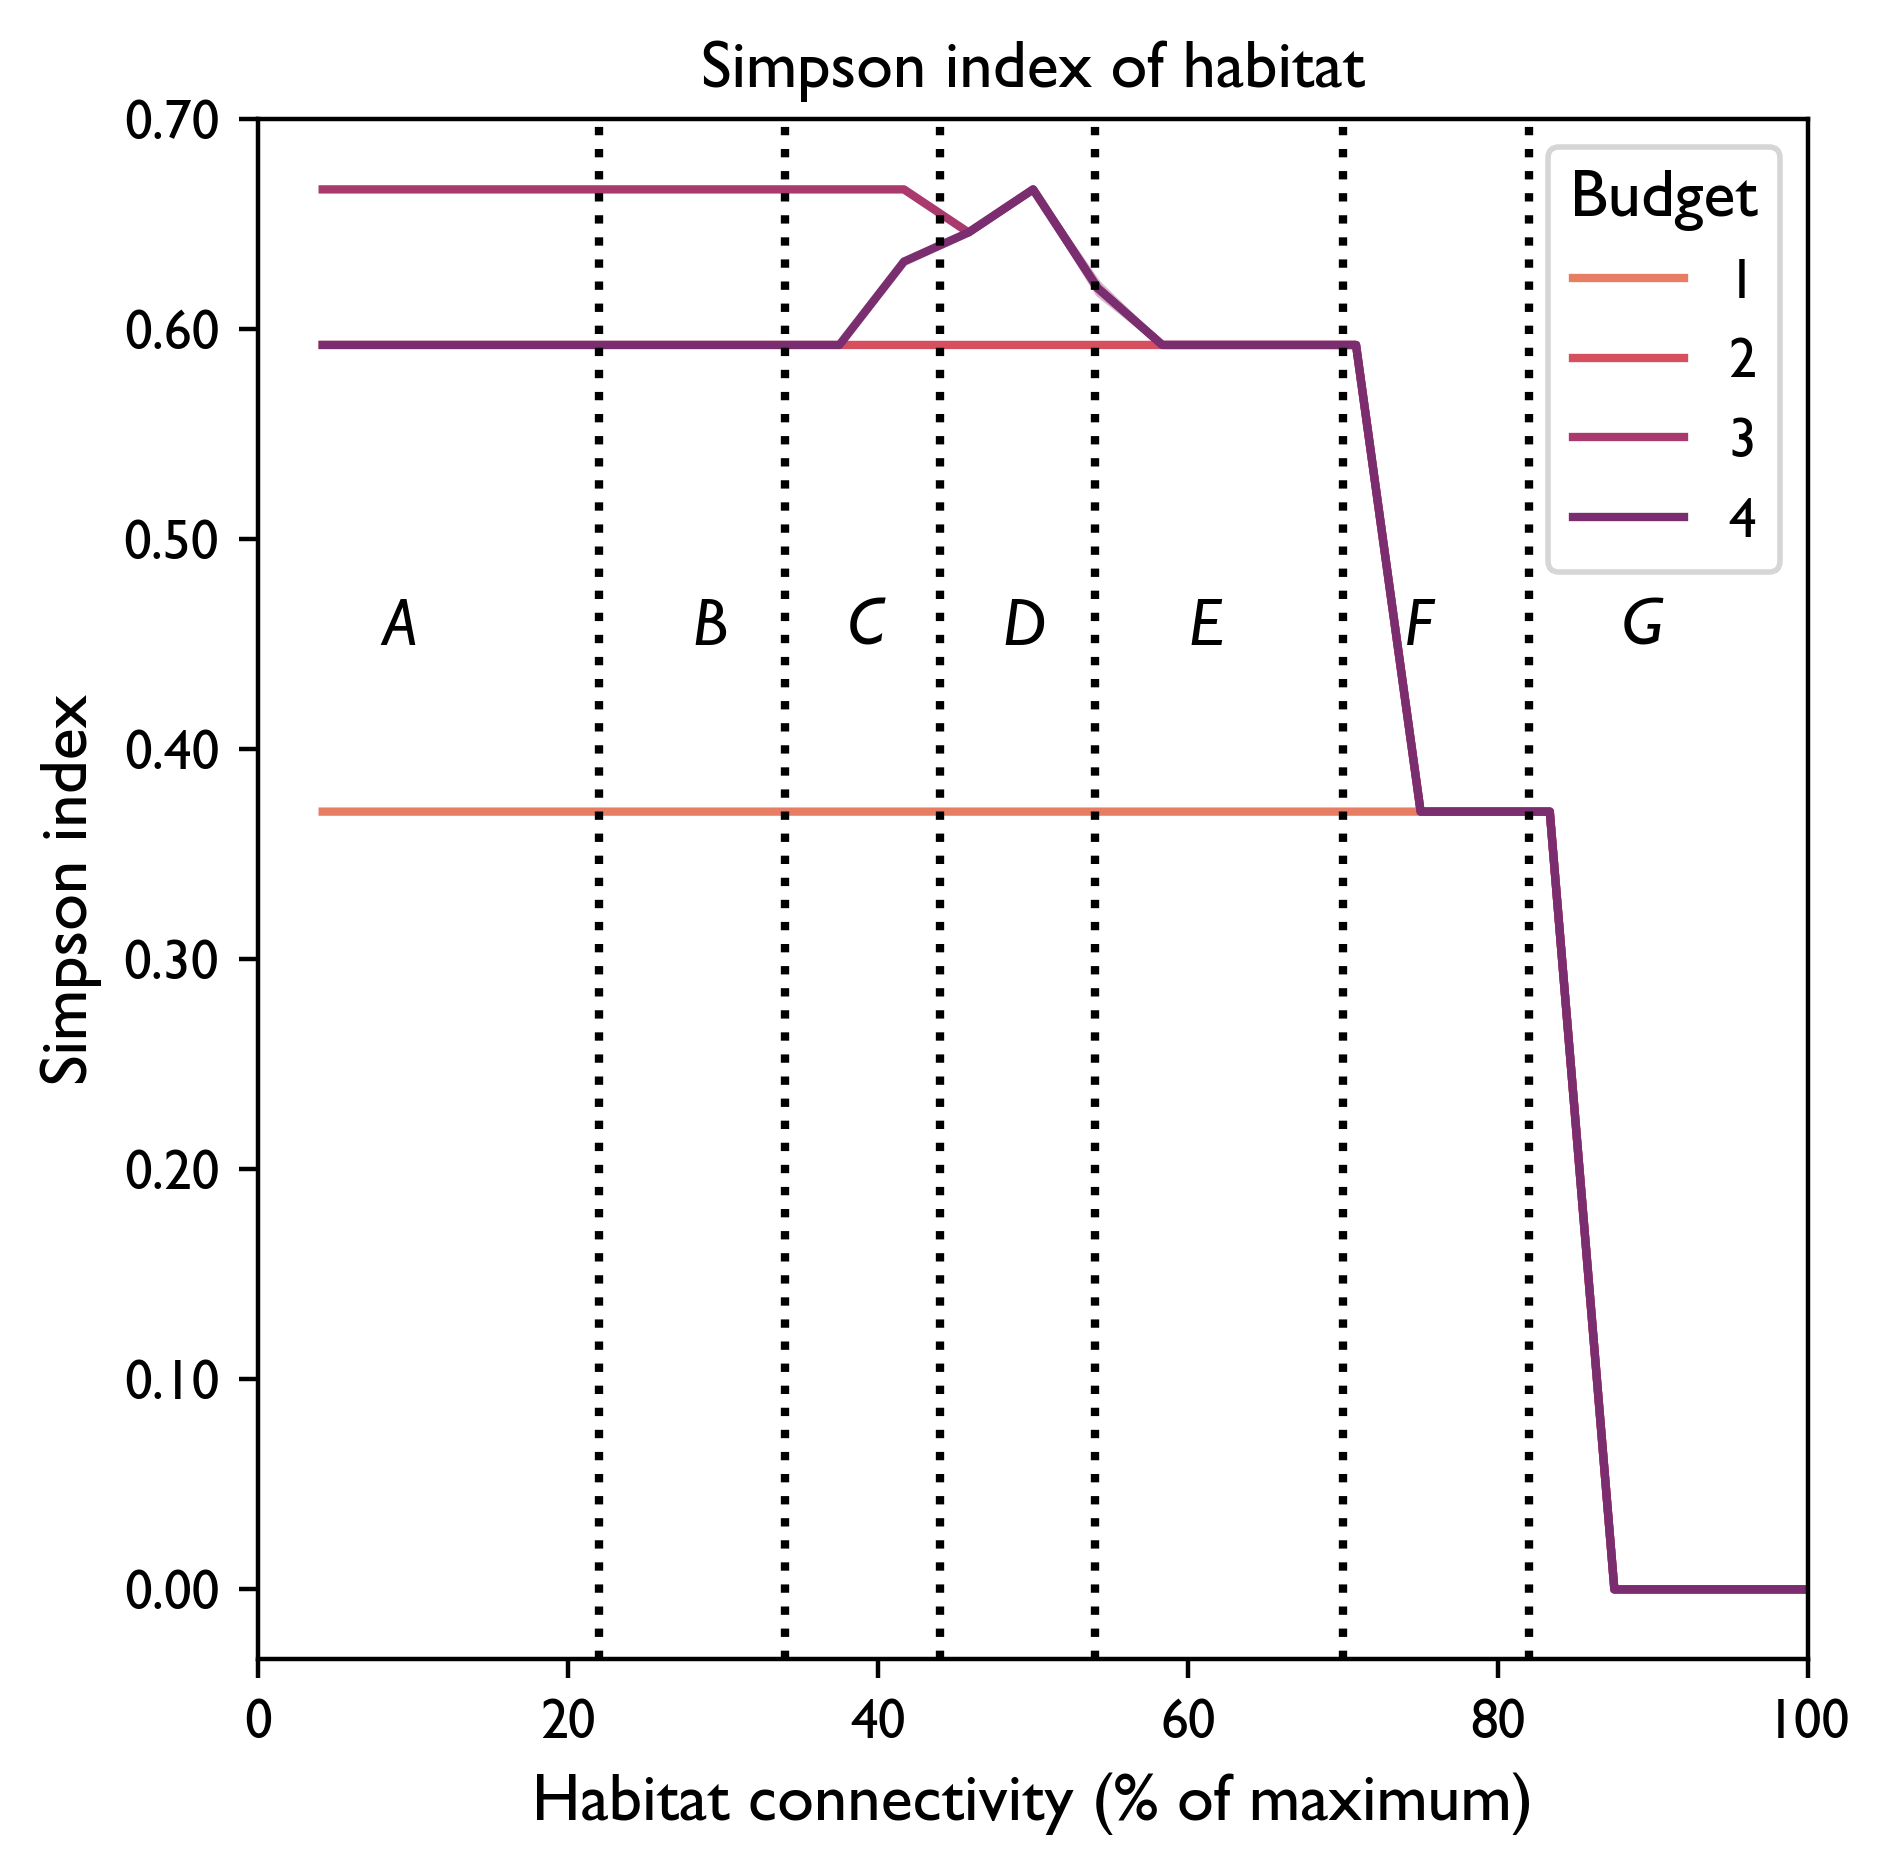
\includegraphics[width=\textwidth]{figures/wildland/simpson_index3.png}
         \caption{}
         \label{fig:indicator_simpson3}
     \end{subfigure}
    \begin{subfigure}[b]{0.4\textwidth}
         \centering
         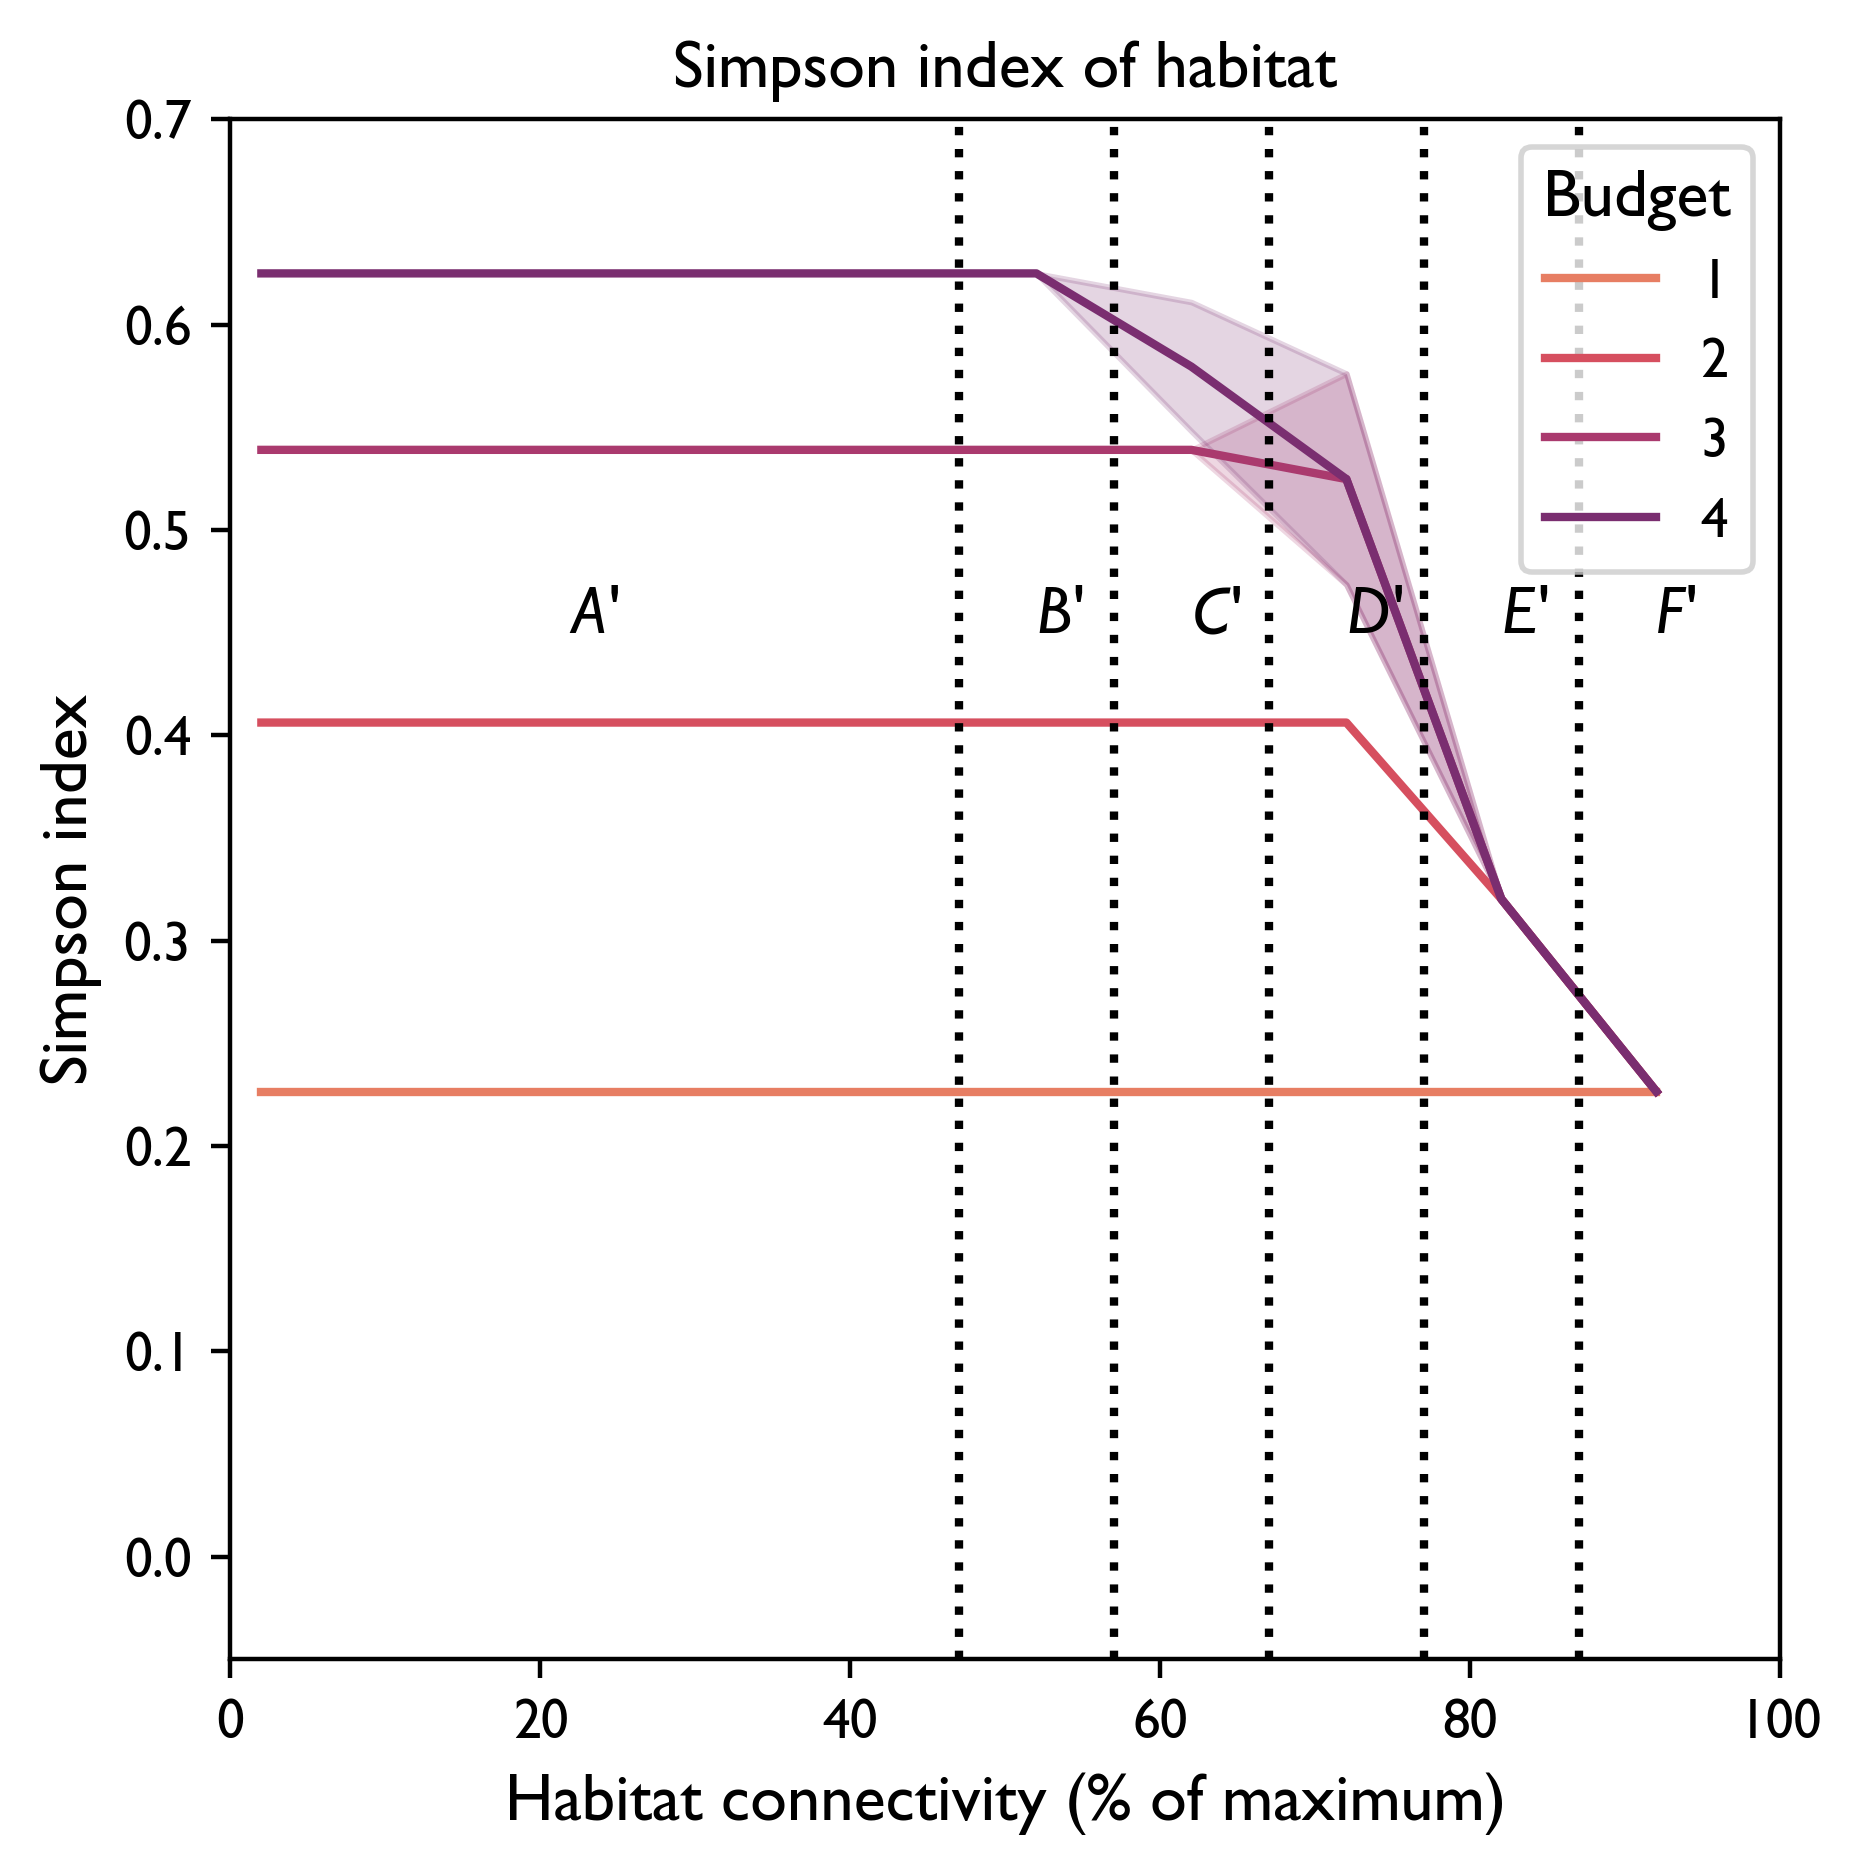
\includegraphics[width=.985\textwidth]{figures/wildland/simpson_index4.png}
         \caption{}
         \label{fig:indicator_simpson4}
    \end{subfigure}
    \hfill
     \begin{subfigure}[b]{0.4\textwidth}
         \centering
         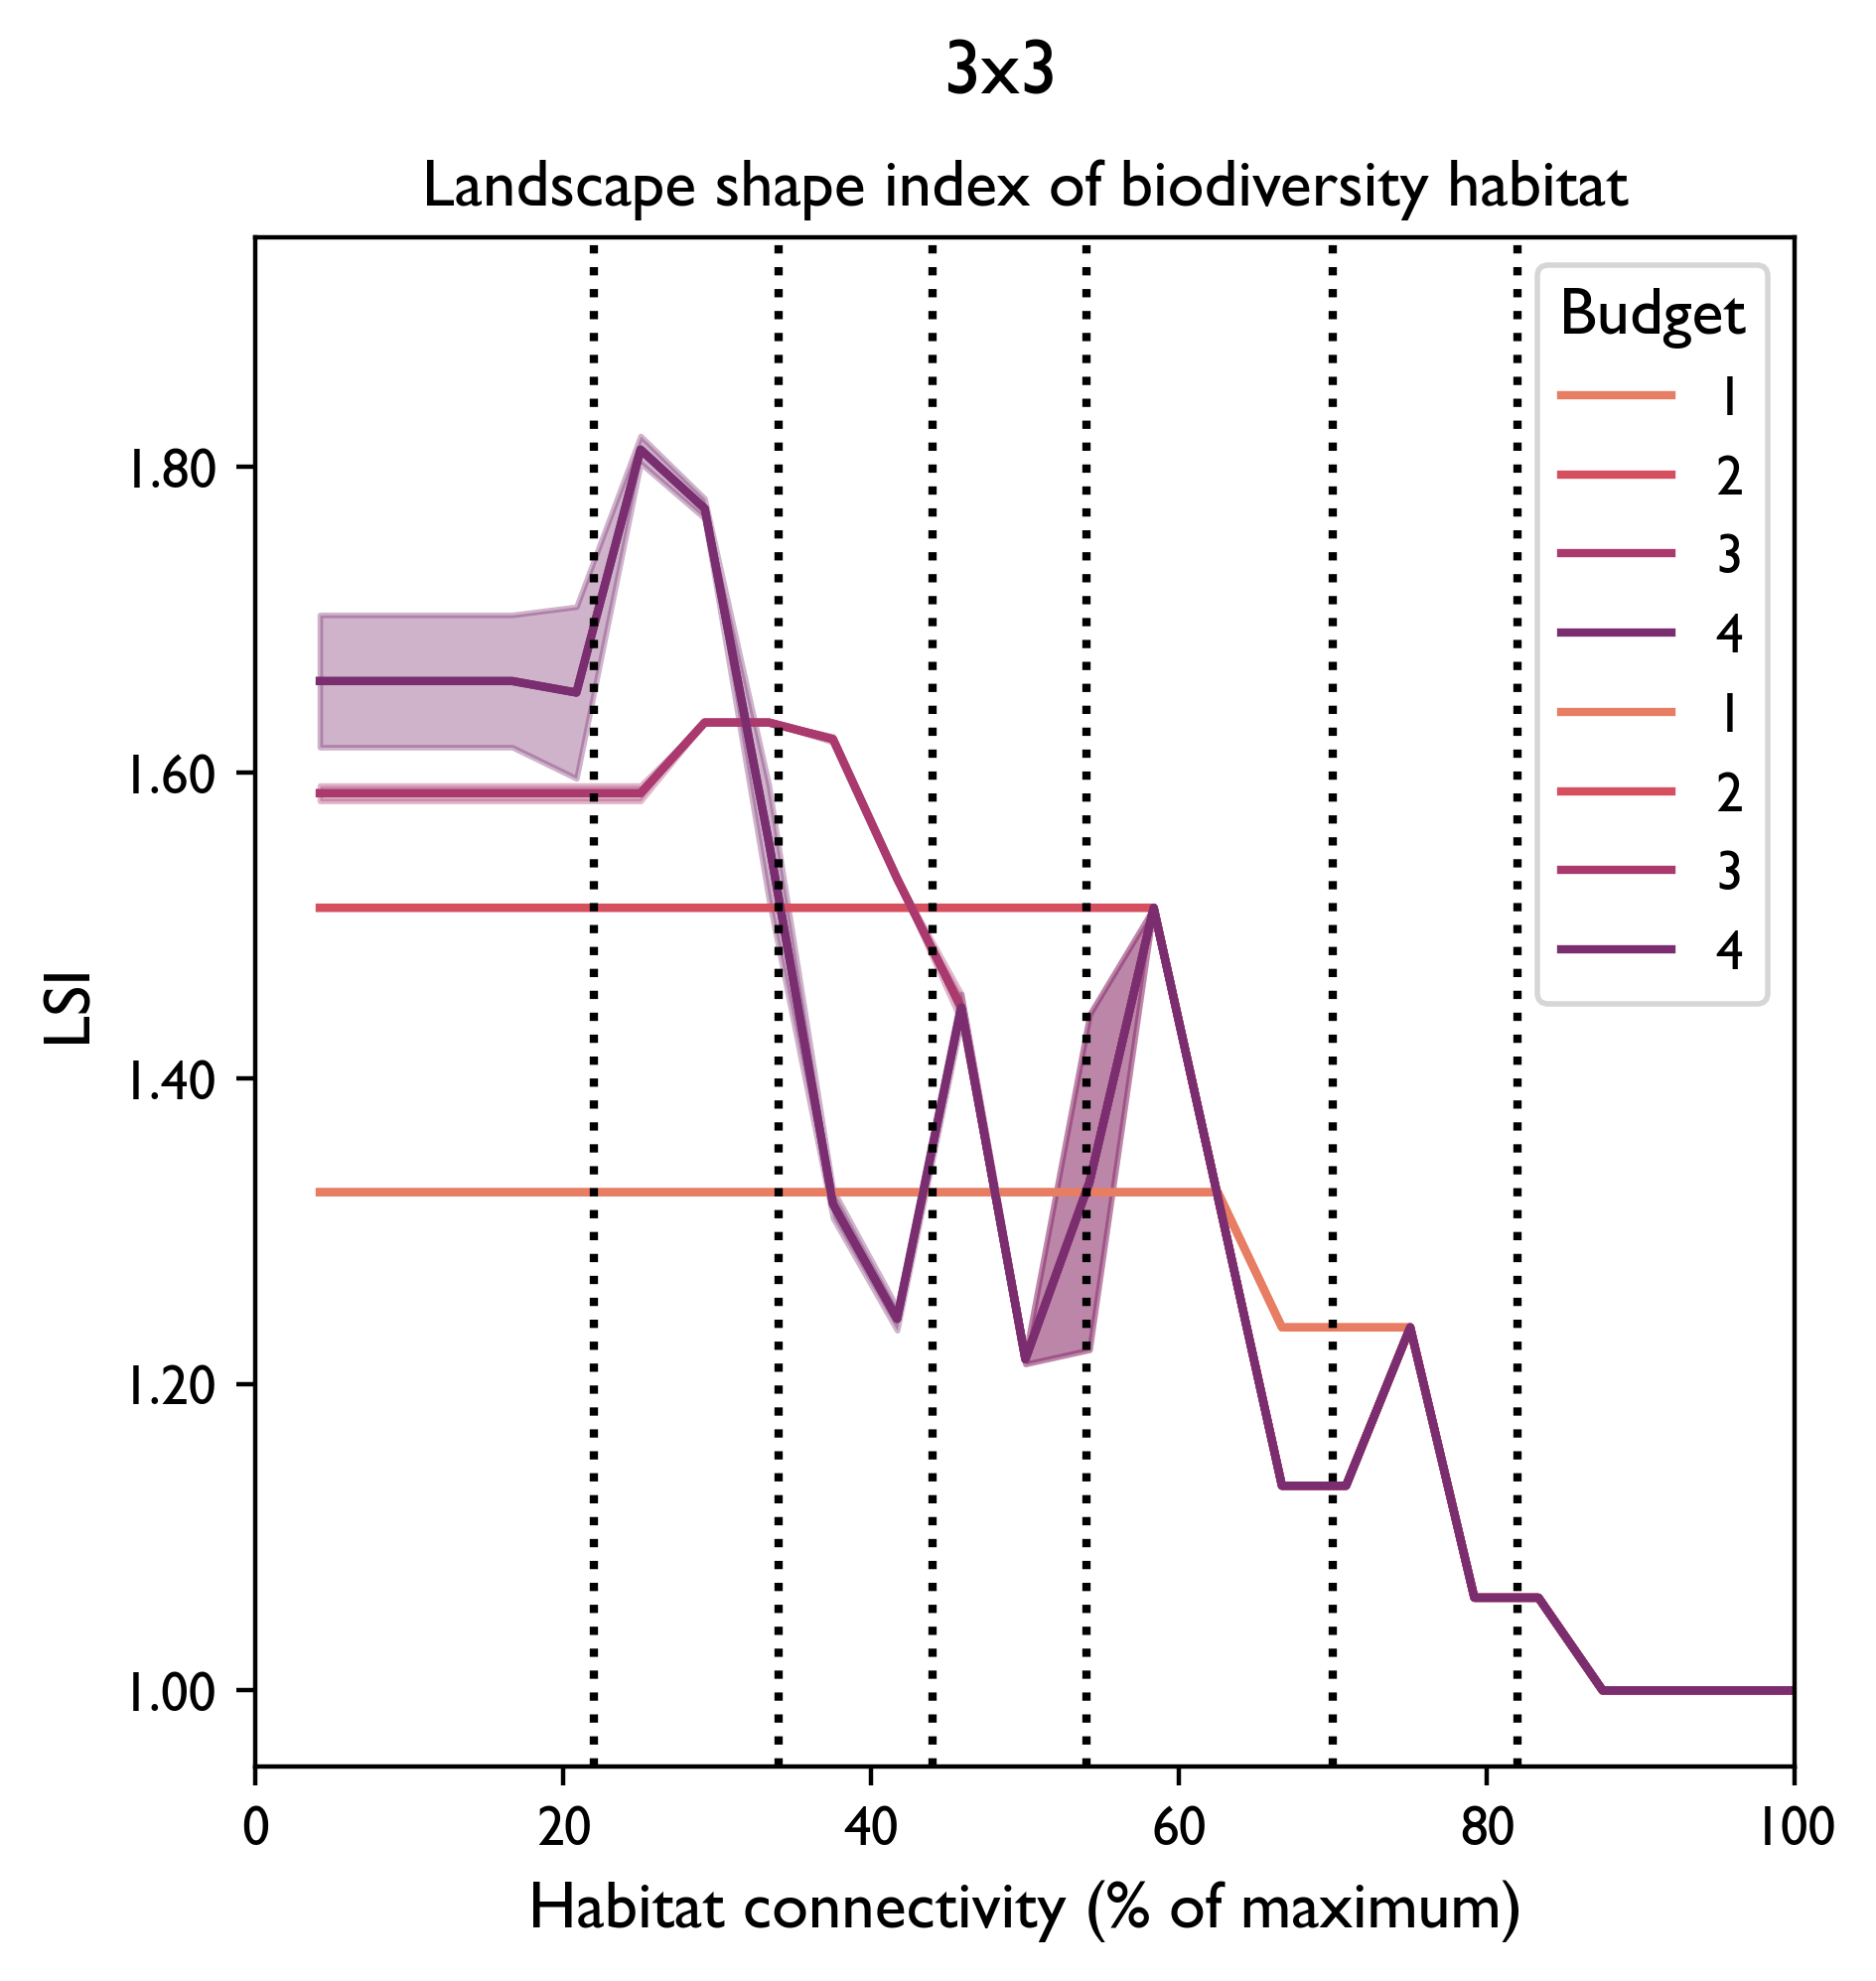
\includegraphics[width=\textwidth]{figures/wildland/LSI_biod3.png}
         \caption{}
         \label{fig:indicator_LSI3}
     \end{subfigure}
     \begin{subfigure}[b]{0.4\textwidth}
         \centering
         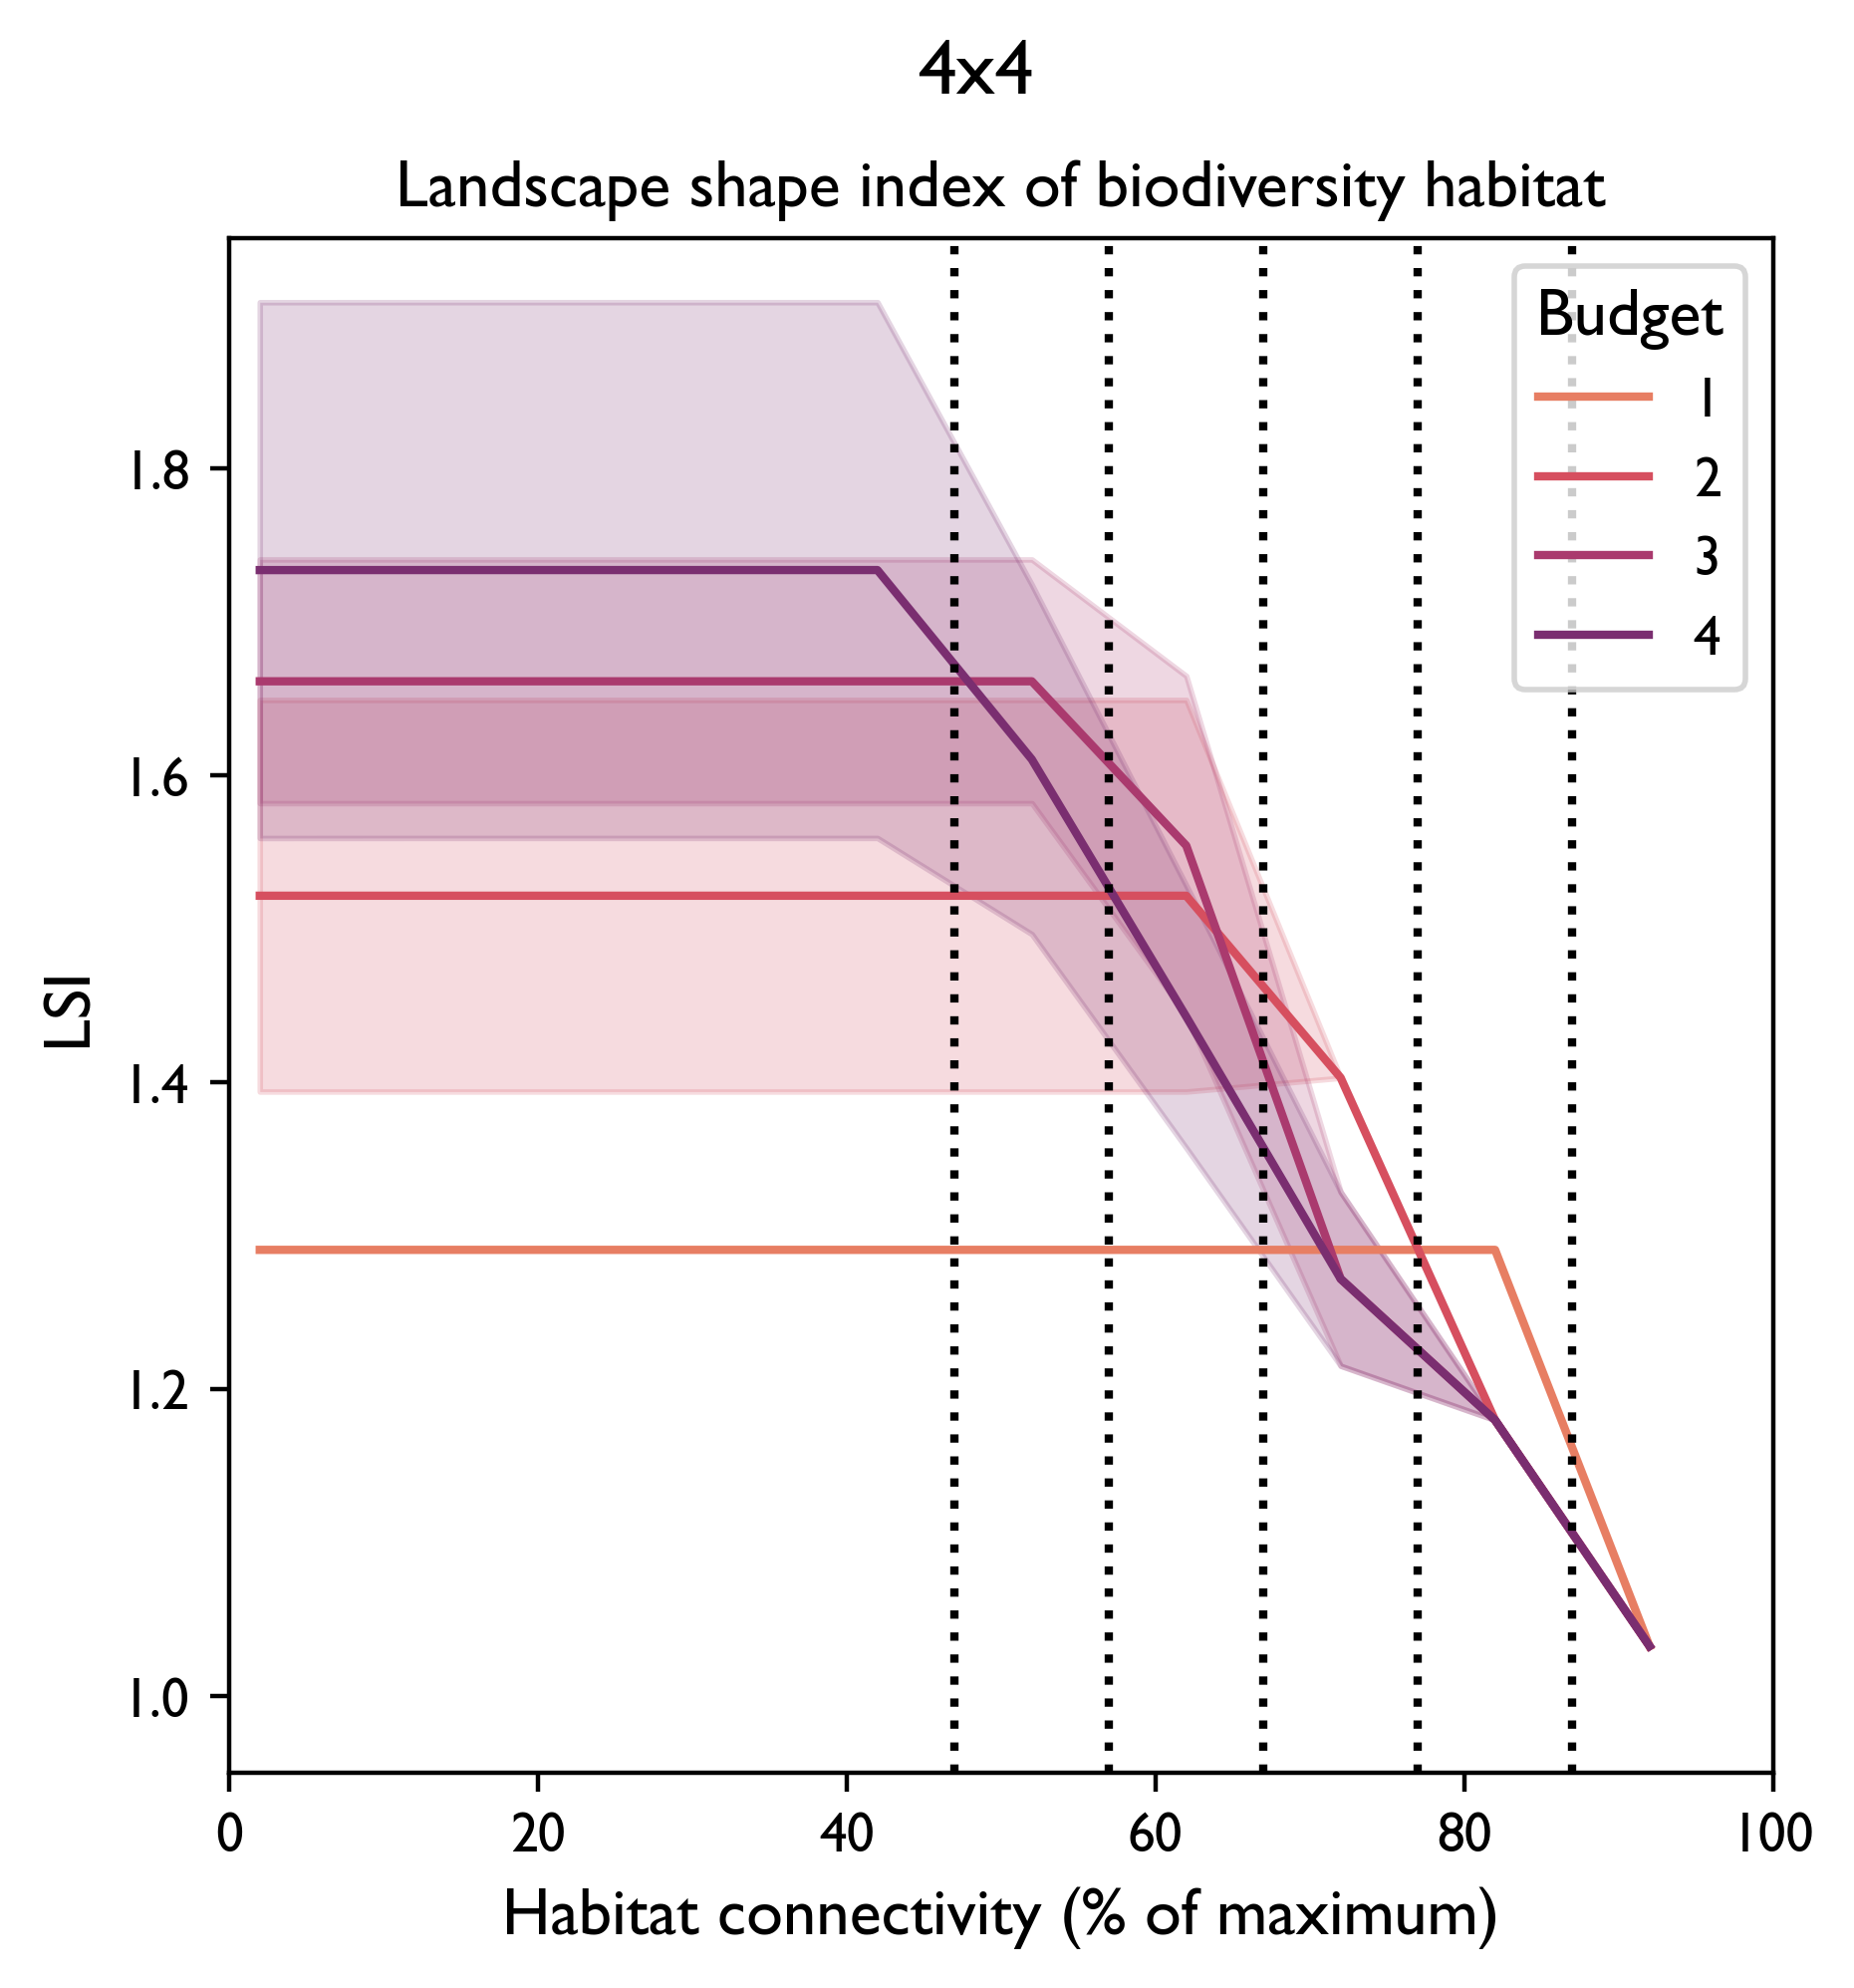
\includegraphics[width=.985\textwidth]{figures/wildland/LSI_biod4.png}
         \caption{}
         \label{fig:indicator_LSI4}
     \end{subfigure}    
    \hfill
    \begin{subfigure}[b]{0.4\textwidth}
         \centering
         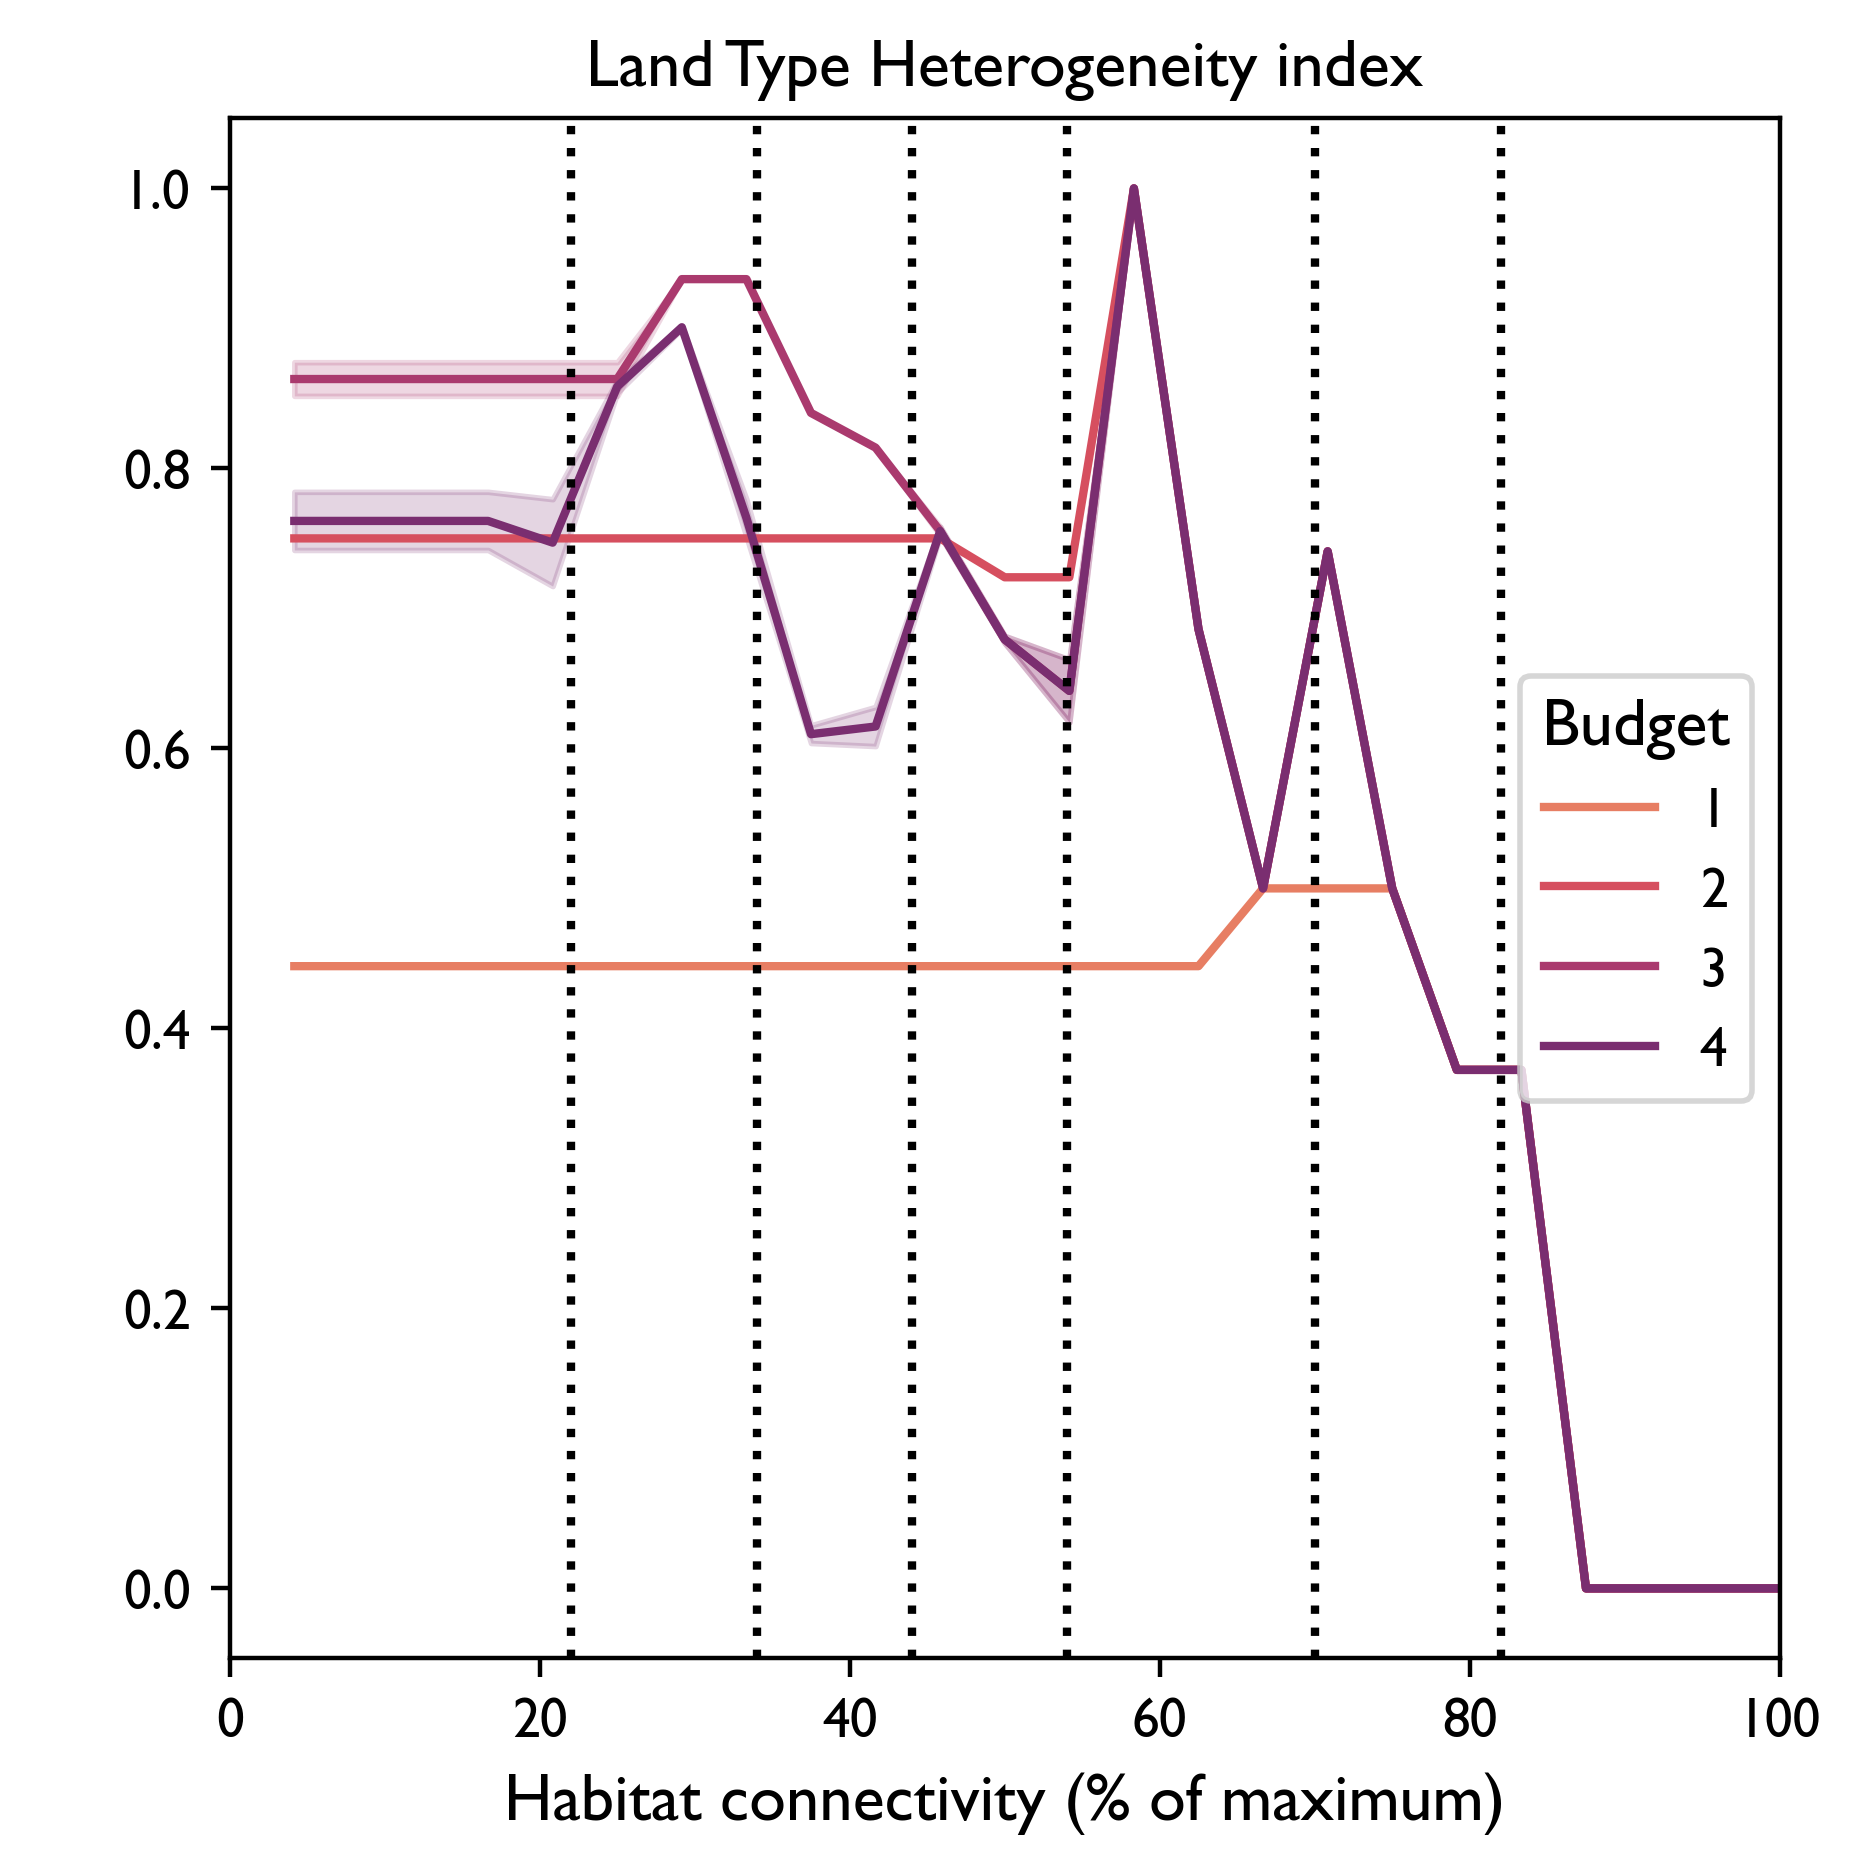
\includegraphics[width=\textwidth]{figures/wildland/diversity_index3.png}
         \caption{}
         \label{fig:indicator_diversity3}
     \end{subfigure}
    \begin{subfigure}[b]{0.4\textwidth}
         \centering
         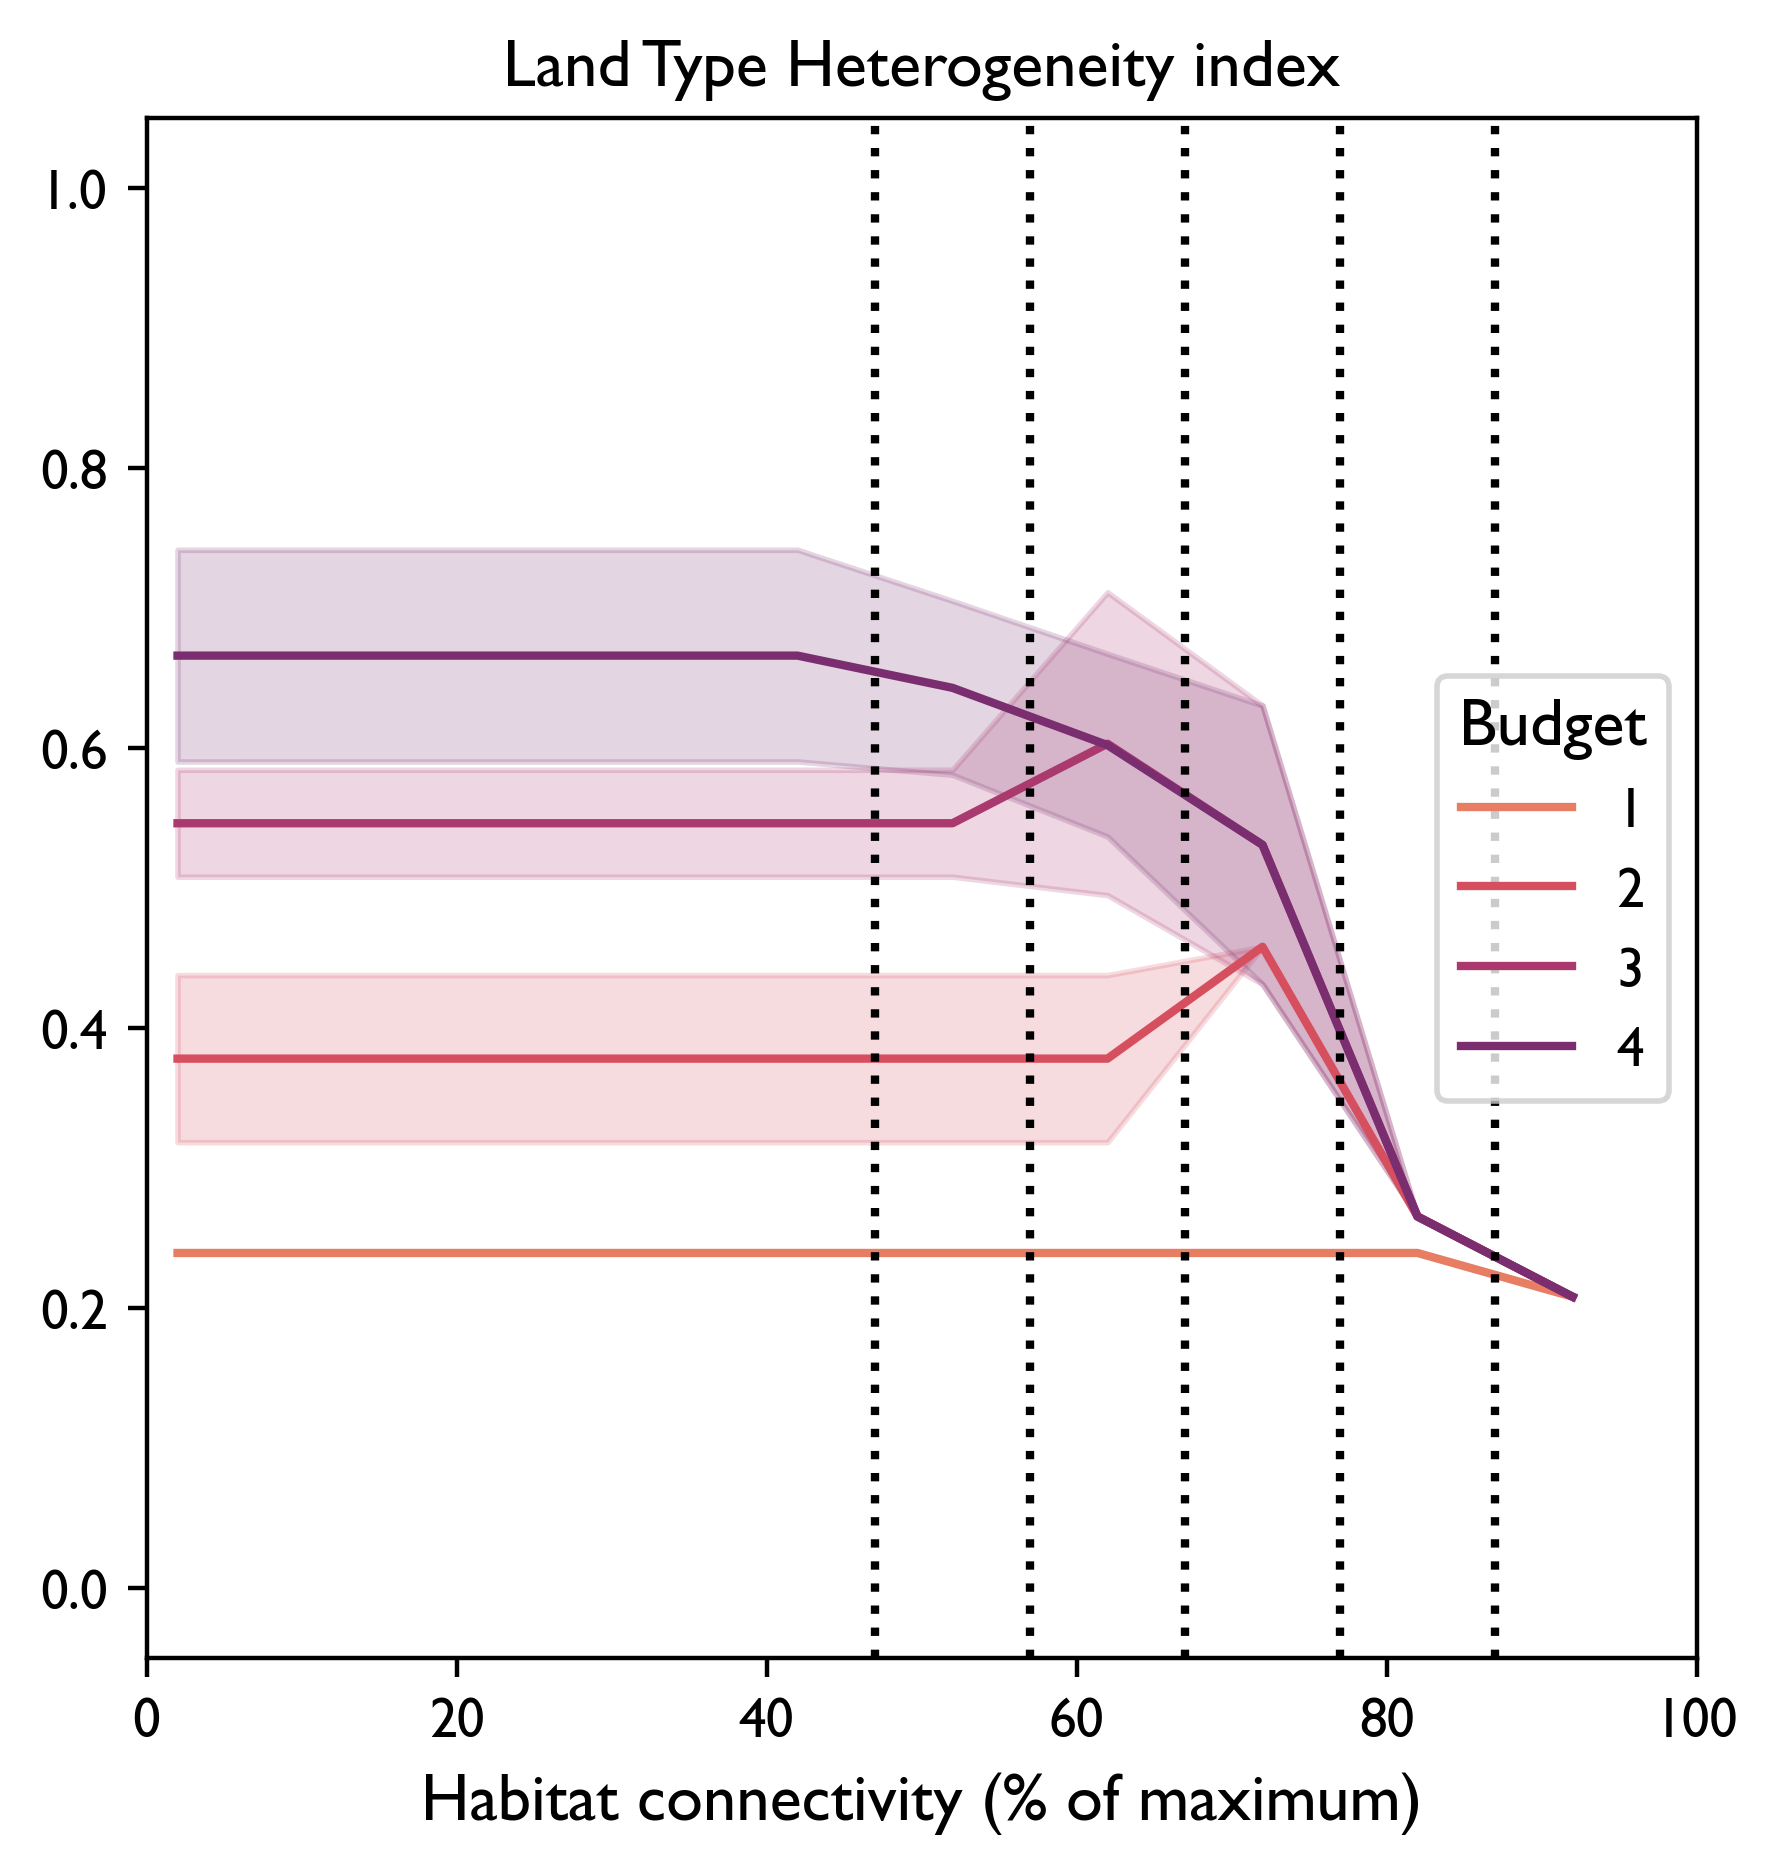
\includegraphics[width=0.955\textwidth]{figures/wildland/diversity_index4.png}
         \caption{}
         \label{fig:indicator_diversity4}
    \end{subfigure}
        \caption{Assessment: diversity (95\% CI shaded)}
        \label{fig:indicators_2}
\end{figure}
\newpage


% Treatments 
\begin{figure}[H]
     \centering
     \begin{subfigure}[b]{0.48\textwidth}
         \centering
         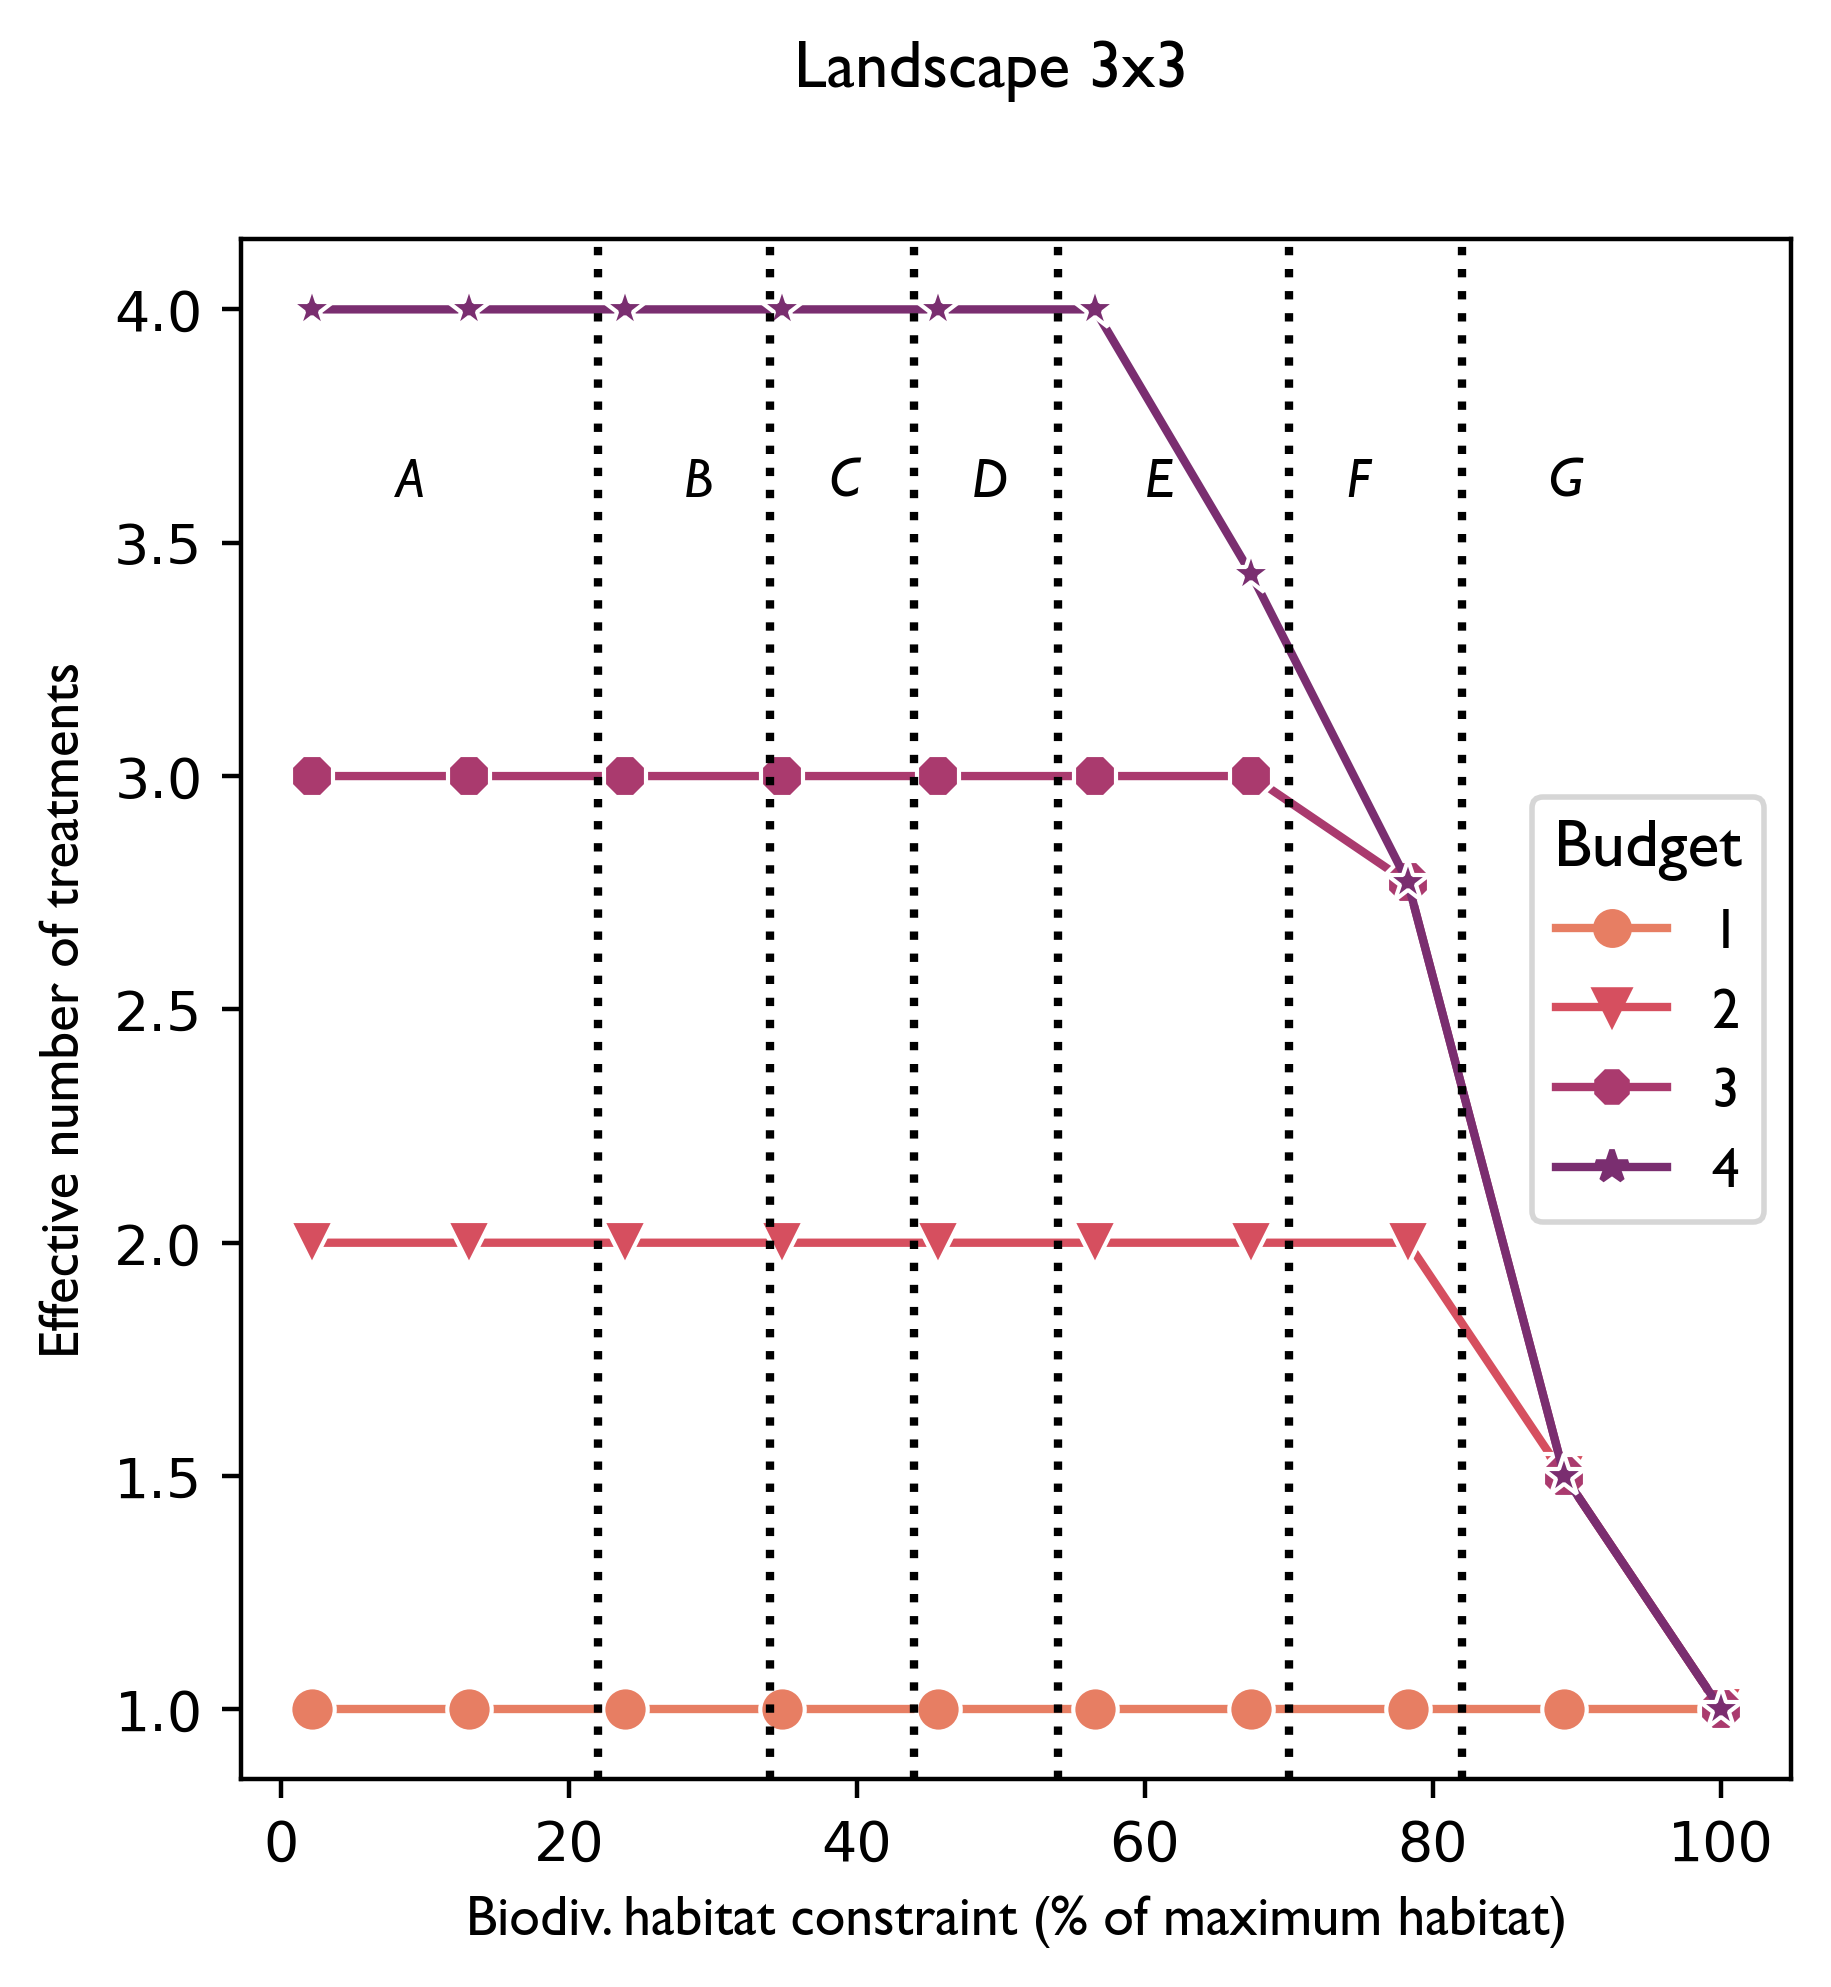
\includegraphics[width=\textwidth]{figures/wildland/number_treatments3.png}
         \caption{}
         \label{fig:treatments_number3}
     \end{subfigure}
    \begin{subfigure}[b]{0.48\textwidth}
         \centering
         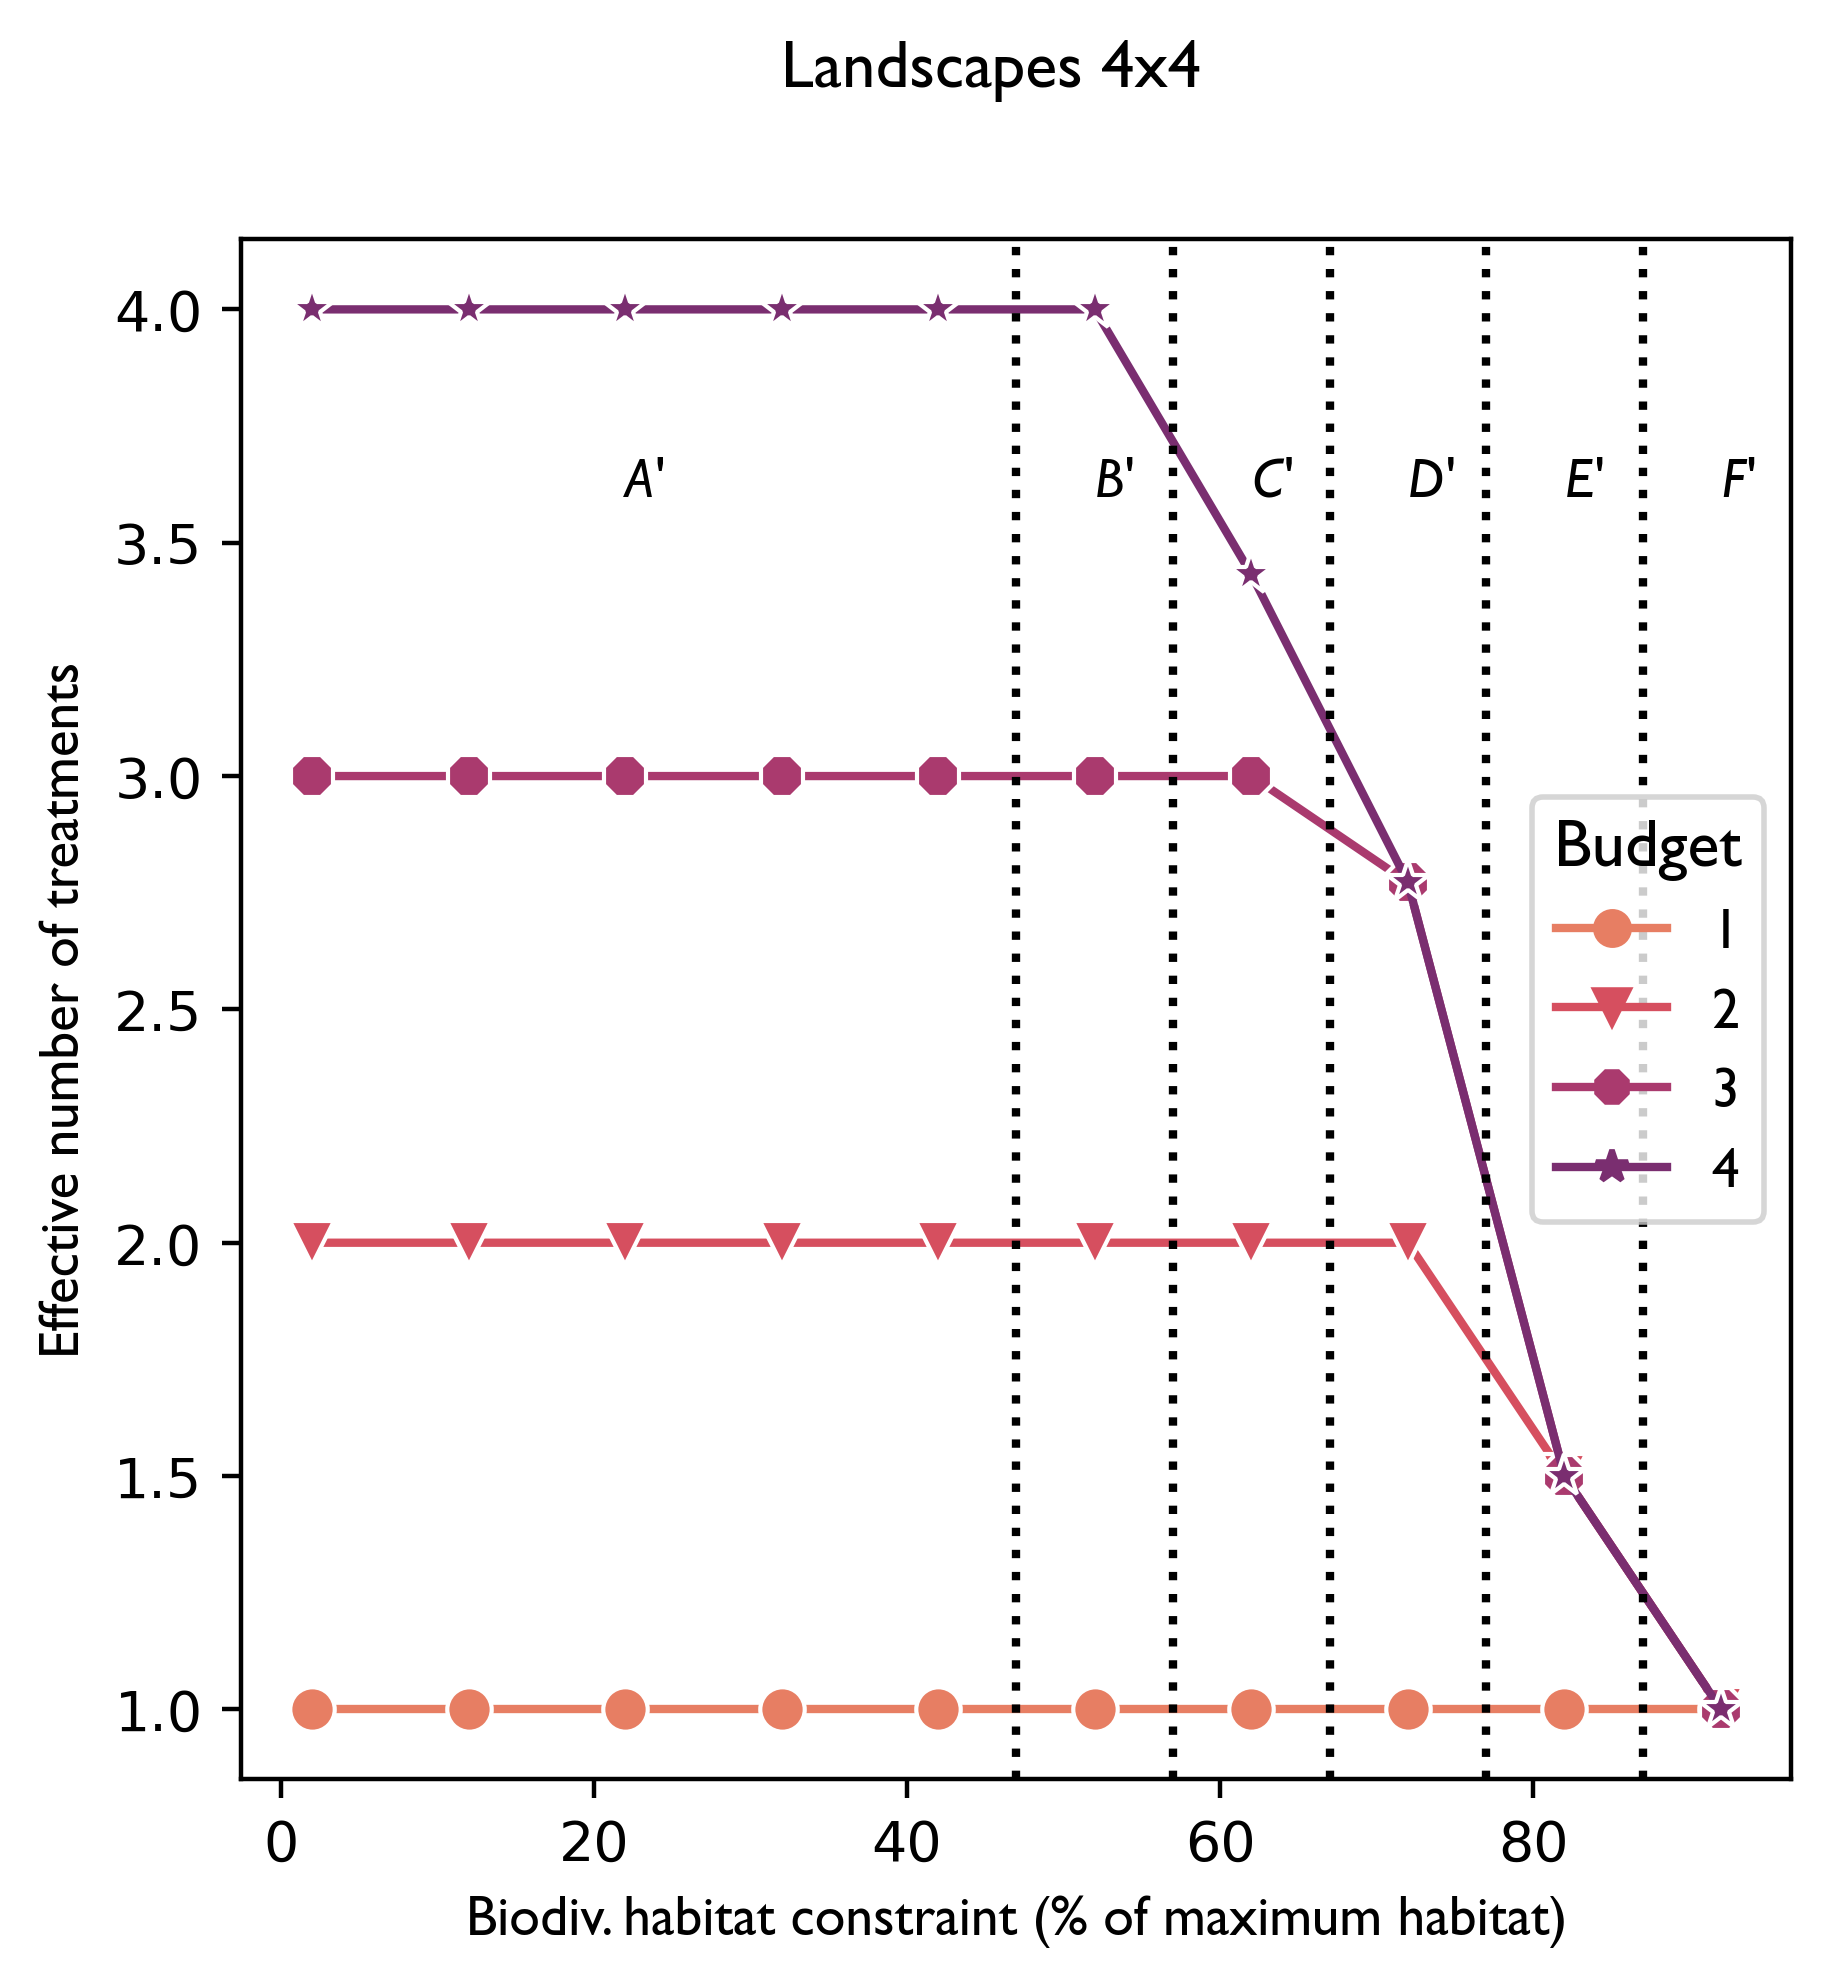
\includegraphics[width=\textwidth]{figures/wildland/number_treatments4.png}
         \caption{}
         \label{fig:treatments_number4}
    \end{subfigure}
    \hfill
     \begin{subfigure}[b]{0.44\textwidth}
         \centering
         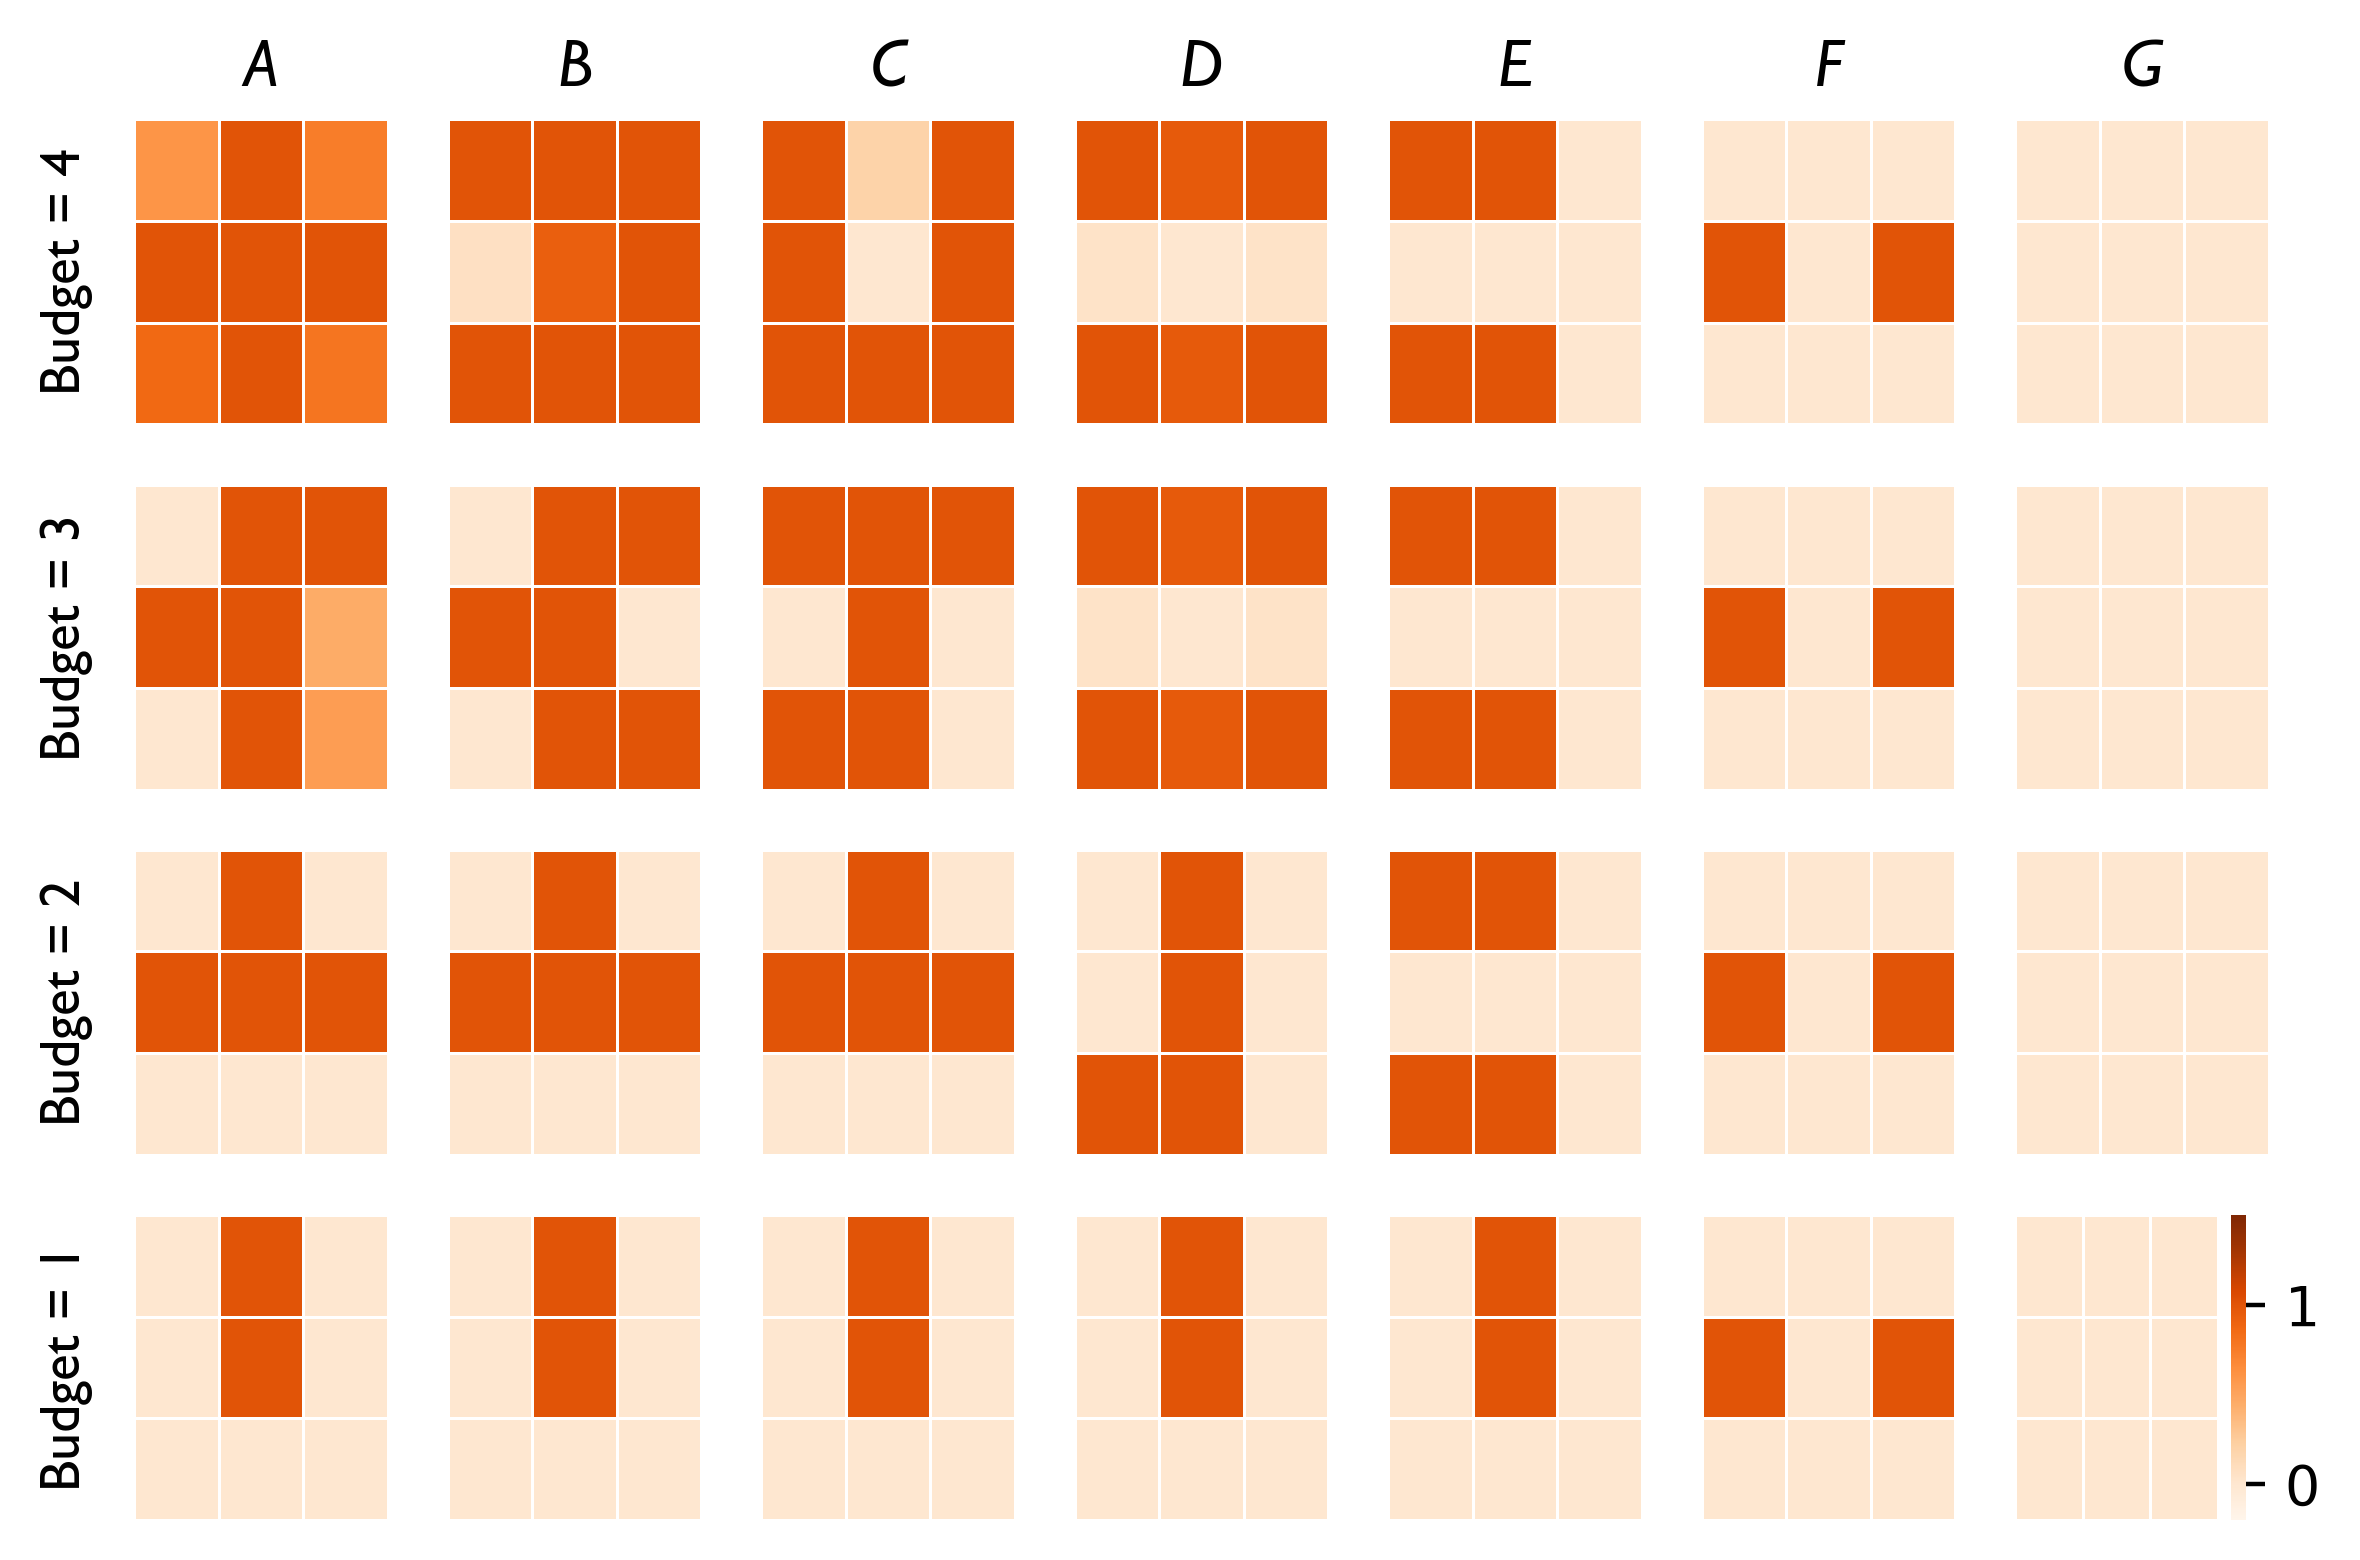
\includegraphics[width=\textwidth]{figures/wildland/treatments3.png}
         \caption{}
         \label{fig:treatments_pattern3}
     \end{subfigure}
     \begin{subfigure}[b]{0.44\textwidth}
         \centering
         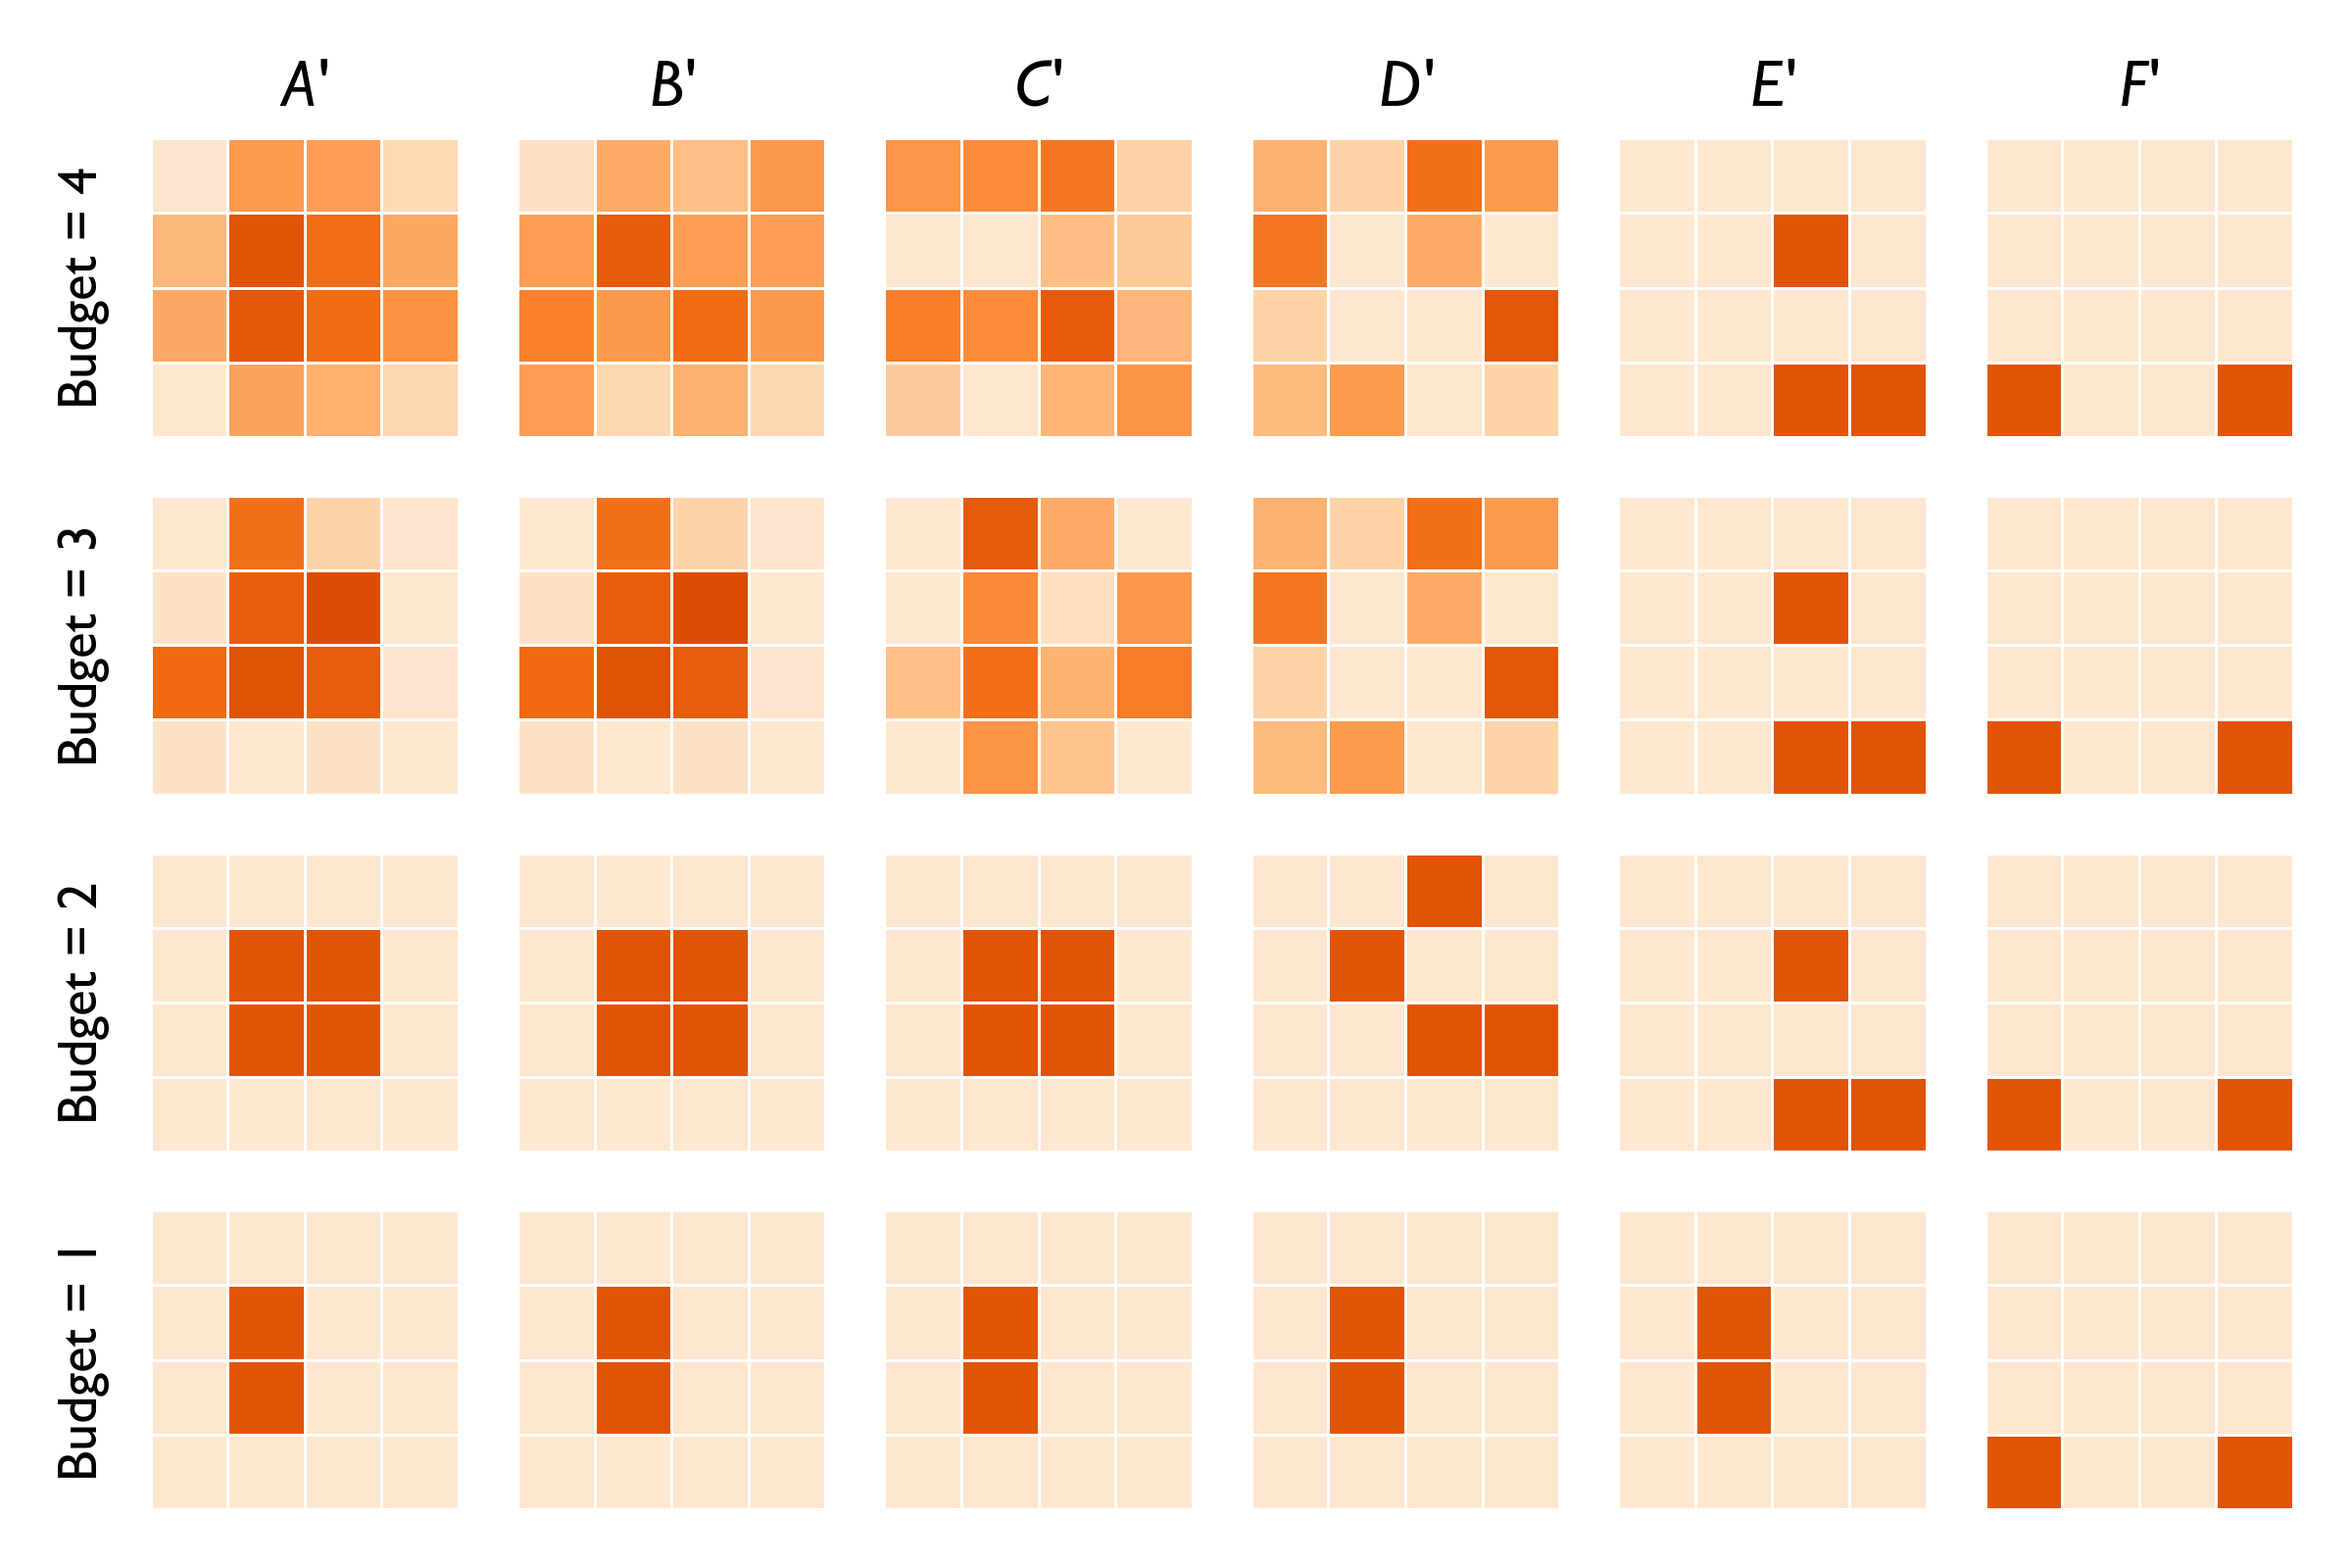
\includegraphics[width=\textwidth]{figures/wildland/treatments4.png}
         \caption{}
         \label{fig:treatments_pattern4}
     \end{subfigure}    
        \caption{Treatment allocation : number, location}
        \label{fig:treatments}
\end{figure}